\documentclass[Review,times,sageh]{sagej}

\usepackage{moreverb,url,natbib, multirow, tabularx}
\usepackage[hidelinks,bookmarksopen,bookmarksnumbered,citecolor=red,urlcolor=red]{hyperref}


% Pandoc citation processing

\usepackage{cleveref}
\providecommand{\tightlist}{\setlength{\itemsep}{0pt}\setlength{\parskip}{0pt}}

\usepackage{booktabs}
\usepackage{longtable}
\usepackage{array}
\usepackage{multirow}
\usepackage{wrapfig}
\usepackage{float}
\usepackage{colortbl}
\usepackage{pdflscape}
\usepackage{tabu}
\usepackage{threeparttable}
\usepackage{threeparttablex}
\usepackage[normalem]{ulem}
\usepackage{makecell}
\usepackage{xcolor}


\begin{document}

\title{Multidimensional signals and analytic flexibility: Estimating degrees of freedom in human speech analyses}

\runninghead{Multidimensional signals and analytic flexibility}

\author{Stefano Coretta*\affilnum{1, 2}, Joseph V. Casillas\affilnum{3}, Simon Roessig\affilnum{4}, Michael Franke\affilnum{5}, Byron Ahn\affilnum{6}, Ali H. Al-Hoorie\affilnum{7}, Jalal Al-Tamimi\affilnum{8}, Najd E. Alotaibi\affilnum{9}, Mohammed K. AlShakhori\affilnum{10}, Ruth M. Altmiller\affilnum{11}, Pablo Arantes\affilnum{12}, Angeliki Athanasopoulou\affilnum{13}, Melissa M. Baese-Berk\affilnum{14}, George Bailey\affilnum{15}, Cheman Baira A Sangma\affilnum{16}, Eleonora J. Beier\affilnum{17}, Gabriela M. Benavides\affilnum{18}, Nicole Benker\affilnum{19}, Emelia P. BensonMeyer\affilnum{20}, Nina R. Benway\affilnum{21}, Grant M. Berry\affilnum{22}, Liwen Bing\affilnum{23}, Christina Bjorndahl\affilnum{24}, Mariska Bolyanatz\affilnum{25}, Aaron Braver\affilnum{26}, Violet A. Brown\affilnum{27}, Alicia M. Brown\affilnum{28}, Alejna Brugos\affilnum{29}, Erin M. Buchanan\affilnum{30}, Tanna Butlin\affilnum{31}, Andrés Buxó-Lugo\affilnum{32}, Coline Caillol\affilnum{33}, Francesco Cangemi\affilnum{34}, Christopher Carignan\affilnum{35}, Sita Carraturo\affilnum{36}, Tiphaine Caudrelier\affilnum{37}, Eleanor Chodroff\affilnum{38}, Michelle Cohn\affilnum{39}, Johanna Cronenberg\affilnum{40}, Olivier Crouzet\affilnum{41}, Erica L. Dagar\affilnum{42}, Charlotte Dawson\affilnum{43}, Carissa A. Diantoro\affilnum{44}, Marie Dokovova\affilnum{45}, Shiloh Drake\affilnum{46}, Fengting Du\affilnum{47}, Margaux Dubuis\affilnum{48}, Florent Duême\affilnum{49}, Matthew Durward\affilnum{50}, Ander Egurtzegi\affilnum{51}, Mahmoud M. Elsherif\affilnum{52}, Janina Esser\affilnum{53}, Emmanuel Ferragne\affilnum{54}, Fernanda Ferreira\affilnum{55}, Lauren K. Fink\affilnum{56}, Sara Finley\affilnum{57}, Kurtis Foster\affilnum{58}, Paul Foulkes\affilnum{59}, Rosa Franzke\affilnum{60}, Gabriel Frazer-McKee\affilnum{61}, Robert Fromont\affilnum{62}, Christina García\affilnum{63}, Jason Geller\affilnum{64}, Camille L. Grasso\affilnum{65}, Pia Greca\affilnum{66}, Martine Grice\affilnum{67}, Magdalena S. Grose-Hodge\affilnum{68}, Amelia J. Gully\affilnum{69}, Caitlin Halfacre\affilnum{70}, Ivy Hauser\affilnum{71}, Jen Hay\affilnum{72}, Robert Haywood\affilnum{73}, Sam Hellmuth\affilnum{74}, Allison I. Hilger\affilnum{75}, Nicole Holliday\affilnum{76}, Damar Hoogland\affilnum{77}, Yaqian Huang\affilnum{78}, Vincent Hughes\affilnum{79}, Ane Icardo Isasa\affilnum{80}, Zlatomira G. Ilchovska\affilnum{81}, Hae-Sung Jeon\affilnum{82}, Jacq Jones\affilnum{83}, Mágat N. Junges\affilnum{84}, Stephanie Kaefer\affilnum{85}, Constantijn Kaland\affilnum{86}, Matthew C. Kelley\affilnum{87}, Niamh E. Kelly\affilnum{88}, Thomas Kettig\affilnum{89}, Ghada Khattab\affilnum{90}, Ruud Koolen\affilnum{91}, Emiel Krahmer\affilnum{92}, Dorota Krajewska\affilnum{93}, Andreas Krug\affilnum{94}, Abhilasha A. Kumar\affilnum{95}, Anna Lander\affilnum{96}, Tomas O. Lentz\affilnum{97}, Wanyin Li\affilnum{98}, Yanyu Li\affilnum{99}, Maria Lialiou\affilnum{100}, Ronaldo M. Lima Jr.\affilnum{101}, Justin J. H. Lo\affilnum{102}, Julio Cesar Lopez Otero\affilnum{103}, Bradley Mackay\affilnum{104}, Bethany MacLeod\affilnum{105}, Mel Mallard\affilnum{106}, Carol-Ann Mary McConnellogue\affilnum{107}, George Moroz\affilnum{108}, Mridhula Murali\affilnum{109}, Ladislas Nalborczyk\affilnum{110}, Filip Nenadić\affilnum{111}, Jessica Nieder\affilnum{112}, Dušan Nikolić\affilnum{113}, Francisco G. S. Nogueira\affilnum{114}, Heather M. Offerman\affilnum{115}, Elisa Passoni\affilnum{116}, Maud Pélissier\affilnum{117}, Scott J. Perry\affilnum{118}, Alexandra M. Pfiffner\affilnum{119}, Michael Proctor\affilnum{120}, Ryan Rhodes\affilnum{121}, Nicole Rodríguez\affilnum{122}, Elizabeth Roepke\affilnum{123}, Jan P. Röer\affilnum{124}, Lucia Sbacco\affilnum{125}, Rebecca Scarborough\affilnum{126}, Felix Schaeffler\affilnum{127}, Erik Schleef\affilnum{128}, Dominic Schmitz\affilnum{129}, Alexander Shiryaev\affilnum{130}, Márton Sóskuthy\affilnum{131}, Malin Spaniol\affilnum{132}, Joseph A. Stanley\affilnum{133}, Alyssa Strickler\affilnum{134}, Alessandro Tavano\affilnum{135}, Fabian Tomaschek\affilnum{136}, Benjamin V. Tucker\affilnum{137}, Rory Turnbull\affilnum{138}, Kingsley O. Ugwuanyi\affilnum{139}, Iñigo Urrestarazu-Porta\affilnum{140}, Ruben van de Vijver\affilnum{141}, Kristin J. Van Engen\affilnum{142}, Emiel van Miltenburg\affilnum{143}, Bruce Wang\affilnum{144}, Natasha Warner\affilnum{145}, Simon Wehrle\affilnum{146}, Hans Westerbeek\affilnum{147}, Seth Wiener\affilnum{148}, Stephen Winters\affilnum{149}, Sidney G.-J. Wong\affilnum{150}, Anna Wood\affilnum{151}, Jane Wottawa\affilnum{152}, Chenzi Xu\affilnum{153}, Germán Zárate-Sández\affilnum{154}, Georgia Zellou\affilnum{155}, Cong Zhang\affilnum{156}, Jian Zhu\affilnum{157}, Timo B. Roettger\affilnum{158}}

\affiliation{\affilnum{1, 2}{Department of Linguistics and English Language, University of Edinburgh, United Kingdom}\\\affilnum{3}{Department of Spanish and Portuguese, Rutgers University, United States}\\\affilnum{4}{Department of Linguistics, Cornell University, United States}\\\affilnum{5}{Department of General and Computational Linguistics, University of Tübingen, Germany}\\\affilnum{6}{Program in Linguistics, Princeton University, United States}\\\affilnum{7}{Jubail English Language and Preparatory Year Institute, Royal Commission for Jubail and Yanbu, Saudi Arabia}\\\affilnum{8}{Laboratoire de Lingusitique Formelle (LLF), CNRS, Université Paris Cité, France}\\\affilnum{9}{School of Education, Communication and Language Studies - ECLS, Newcastle University, United Kingdom}\\\affilnum{10}{Department of Linguistics, University of Arizona, United States}\\\affilnum{11}{Psychological and Brain Sciences, Washington University in Saint Louis, United States}\\\affilnum{12}{Departamento de Letras, Universidade Federal de São Carlos, Brazil}\\\affilnum{13}{School of Languages, Linguistics, Literatures and Cultures, University of Calgary, Canada}\\\affilnum{14}{Department of Linguistics, University of Oregon, United States}\\\affilnum{15}{Department of Language and Linguistic Science, University of York, United Kingdom}\\\affilnum{16}{School of Languages, Linguistics, Literatures and Cultures, University of Calgary, Canada}\\\affilnum{17}{Department of Psychology, University of California, Davis, United States}\\\affilnum{18}{Department of Linguistics, University of Arizona, United States}\\\affilnum{19}{Institute of Phonetics and Speech Processing, University of Munich, Germany}\\\affilnum{20}{University of Pennsylvania, United States}\\\affilnum{21}{Department of Communication Sciences and Disorders, Syracuse University, United States}\\\affilnum{22}{Department of Spanish, Villanova University, United States}\\\affilnum{23}{Department of English Language and Linguistics, University of Birmingham, United Kingdom}\\\affilnum{24}{Department of Philosophy, Carnegie Mellon University, United States}\\\affilnum{25}{Department of Spanish \& French Studies, Occidental College, United States}\\\affilnum{26}{Department of English, Texas Tech University, United States}\\\affilnum{27}{Psychological and Brain Sciences, Washington University in Saint Louis, United States}\\\affilnum{28}{Department of Spanish and Portuguese, University of Arizona, United States}\\\affilnum{29}{Division of Mathematics and Computer Science, Simmons University, United States}\\\affilnum{30}{Analytics, Harrisburg University of Science and Technology, United States}\\\affilnum{31}{School of Languages, Linguistics, Literatures and Cultures, University of Calgary, Canada}\\\affilnum{32}{Department of Psychology, University at Buffalo, SUNY, United States}\\\affilnum{33}{Université Paris Cité, France}\\\affilnum{34}{IfL-Phonetik, University of Cologne, Germany}\\\affilnum{35}{Department of Speech, Hearing and Phonetic Sciences, University College London, United Kingdom}\\\affilnum{36}{Psychological and Brain Sciences, Washington University in Saint Louis, United States}\\\affilnum{37}{Basque Center on Cognition Brain and Language, Spain}\\\affilnum{38}{Department of Language and Linguistic Science, University of York, United Kingdom}\\\affilnum{39}{Department of Linguistics, University of California, Davis, United States}\\\affilnum{40}{Institute of Phonetics and Speech Processing, University of Munich, Germany}\\\affilnum{41}{LLING, UMR6310, Nantes Université / CNRS, France}\\\affilnum{42}{Department of Linguisticss and TESOL, University of Texas at Arlington, United States}\\\affilnum{43}{School of Psychology, Newcastle University, United Kingdom}\\\affilnum{44}{Department of Linguistics, University of Oregon, United States}\\\affilnum{45}{School of Psychological Sciences and Health, University of Strathclyde, United Kingdom}\\\affilnum{46}{Department of Linguistics, University of Oregon, United States}\\\affilnum{47}{School of English Literature, Language and Linguistics, Newcastle University, United Kingdom}\\\affilnum{48}{Department of comparative language science, Universität Zürich, Swizerland, Switzerland}\\\affilnum{49}{Basque Center on Cognition Brain and Language, Spain}\\\affilnum{50}{Department of Linguistics, University of Canterbury, New Zealand}\\\affilnum{51}{IKER (UMR 5478), Centre National de la Recherche Scientifique (CNRS), France}\\\affilnum{52}{Department of Neuroscience, Psychology and Behaviour, University of Leicester, United Kingdom}\\\affilnum{53}{Statistics Group, Association for Diversity in Linguistics, Germany}\\\affilnum{54}{CLILLAC-ARP, Université Paris Cité, France}\\\affilnum{55}{Department of Psychology, University of California, Davis, United States}\\\affilnum{56}{Department of Music, Max Planck Institute for Empirical Aesthetics, Germany}\\\affilnum{57}{Department of Psychology, Pacific Lutheran University, United States}\\\affilnum{58}{Department of Linguistics, University of Oregon, United States}\\\affilnum{59}{Department of Language and Linguistic Science, University of York, United Kingdom}\\\affilnum{60}{Institute of Phonetics and Speech Processing, University of Munich, Germany}\\\affilnum{61}{Department of languages, linguistics, and translation, Université Laval, Canada}\\\affilnum{62}{New Zealand Institute of Language, Brain and Behaviour, University of Canterbury, New Zealand}\\\affilnum{63}{Department of Languages, Literatures, and Cultures, Saint Louis University, United States}\\\affilnum{64}{Department of Psychology, Princeton University, United States}\\\affilnum{65}{LPC, Aix Marseille Univ, CNRS, France}\\\affilnum{66}{Institute of Phonetics and Speech Processing, University of Munich, Germany}\\\affilnum{67}{IfL-Phonetik, University of Cologne, Germany}\\\affilnum{68}{Department of English Language and Linguistics, University of Birmingham, United Kingdom}\\\affilnum{69}{Department of Language and Linguistic Science, University of York, United Kingdom}\\\affilnum{70}{School of English Literature, Language and Linguistics, Newcastle University, United Kingdom}\\\affilnum{71}{Department of Linguistics and TESOL, University of Texas at Arlington, United States}\\\affilnum{72}{New Zealand Institute of Language, Brain and Behaviour, University of Canterbury, New Zealand}\\\affilnum{73}{Ao Tawhiti Unlimited Discovery, New Zealand}\\\affilnum{74}{Department of Language and Linguistic Science, University of York, United Kingdom}\\\affilnum{75}{Department of Speech, Language, and Hearing Sciences, University of Colorado Boulder, United States}\\\affilnum{76}{Department of Linguistics and Cognitive Science, Pomona College, United States}\\\affilnum{77}{School of Education, Communication and Language Studies - ECLS, Newcastle University, United Kingdom}\\\affilnum{78}{University of California, Los Angeles, United States}\\\affilnum{79}{Department of Language and Linguistic Science, University of York, United Kingdom}\\\affilnum{80}{Department of Modern and Classical Languages and Literatures, California State University, Northridge, United States}\\\affilnum{81}{School of Psychology, University of Birmingham, United Kingdom}\\\affilnum{82}{School of Humanities, Language and Global Studies, University of Central Lancashire, United Kingdom}\\\affilnum{83}{Department of Linguistics, University of Canterbury, Aotearoa}\\\affilnum{84}{Programa de Pós-Graduação em Letras, Federal University of Rio Grande do Sul, Brazil}\\\affilnum{85}{Department of Linguistics, University of Canterbury, New Zealand}\\\affilnum{86}{Institute of Linguistics, University of Cologne, Germany}\\\affilnum{87}{Department of Linguistics, University of Washington, United States}\\\affilnum{88}{School of English Literature, Language and Linguistics, Newcastle University, United Kingdom}\\\affilnum{89}{Department of Language and Linguistic Science, University of York, United Kingdom}\\\affilnum{90}{School of Education, Communication and Language Studies - ECLS, Newcastle University, United Kingdom}\\\affilnum{91}{Department of Communication and Cognition, Tilburg University, Netherlands}\\\affilnum{92}{Department of Communication and Cognition, Tilburg University, the Netherlands}\\\affilnum{93}{Department of Linguistics and Basque Studies, University of the Basque Country UPV/EHU, Spain}\\\affilnum{94}{School of Education, Communication and Language Studies - ECLS, Newcastle University, United Kingdom}\\\affilnum{95}{Department of Psychology, Bowdoin College, ME, United States}\\\affilnum{96}{Linguistic Convergence Laboratory, HSE University, Russia}\\\affilnum{97}{Department of Communication and Cognition, Tilburg University, the Netherlands}\\\affilnum{98}{School of Psychology, University of Birmingham, United Kingdom}\\\affilnum{99}{School of Education, Communication and Language Studies - ECLS, Newcastle University, United Kingdom}\\\affilnum{100}{Institute of German Language I Linguistics, University of Cologne, Germany}\\\affilnum{101}{Department of English Language Studies, Federal University of Ceará, Brazil}\\\affilnum{102}{Department of Speech, Hearing and Phonetic Sciences, University College London, United Kingdom}\\\affilnum{103}{Department of Hispanic Studies, University of Houston, United States}\\\affilnum{104}{Department of English and American Studies, University of Salzburg, Austria}\\\affilnum{105}{School of Linguistics \& Language Studies, Carleton University, Canada}\\\affilnum{106}{Psychological and Brain Sciences, Washington University in Saint Louis, United States}\\\affilnum{107}{Population Health Sciences Institute - Faculty of Medical Sciences, Newcastle University, United Kingdom}\\\affilnum{108}{HSE University, Russia}\\\affilnum{109}{Speech and Language Therapy, University of Strathclyde, United Kingdom}\\\affilnum{110}{LPC, Aix Marseille Univ, CNRS, France}\\\affilnum{111}{Department of Psychology, Faculty of Media and Communications, Singidunum University, Serbia}\\\affilnum{112}{Institute of Linguistics, Heinrich-Heine University Düsseldorf, Germany}\\\affilnum{113}{School of Languages, Linguistics, Literatures and Cultures, University of Calgary, Canada}\\\affilnum{114}{Graduate Program in Linguistics, Federal University of Ceará, Brazil}\\\affilnum{115}{World Languages, Literatures and Cultures Department, University of Arkansas, United States}\\\affilnum{116}{Deparment of Linguistics, Queen Mary University of London, United Kingdom}\\\affilnum{117}{CLILLAC-ARP, Université Paris Cité, France}\\\affilnum{118}{Department of Linguistics, University of Alberta, Canada}\\\affilnum{119}{Department of Linguistics, University of California, Berkeley, United States}\\\affilnum{120}{Department of Linguistics, Macquarie University, Australia}\\\affilnum{121}{Center for Cognitive Science, Rutgers University, United States}\\\affilnum{122}{Department of Spanish and Portuguese, Rutgers University, United States}\\\affilnum{123}{Department of Speech, Language, and Hearing Sciences, Saint Louis University, United States}\\\affilnum{124}{Department of Psychology, Witten/Herdecke University, Germany}\\\affilnum{125}{School of Education, Communication and Language Studies - ECLS, Newcastle University, United Kingdom}\\\affilnum{126}{Department of Linguistics, University of Colorado Boulder, United States}\\\affilnum{127}{Clinical Audiology, Speech and Language (CASL) Research Centre, Queen Margaret University Edinburgh, United Kingdom}\\\affilnum{128}{Department of English and American Studies, University of Salzburg, Austria}\\\affilnum{129}{Department of English and American Studies, Heinrich Heine University Düsseldorf, Germany}\\\affilnum{130}{Linguistic Convergence Laboratory, HSE University, Russia}\\\affilnum{131}{Department of Linguistics, University of British Columbia, Canada}\\\affilnum{132}{Department of Psychiatry and Psychotherapy, University Hospital Cologne, Germany}\\\affilnum{133}{Department of Linguistics, Brigham Young University, United States}\\\affilnum{134}{Department of Linguistics, University of Colorado Boulder, United States}\\\affilnum{135}{Department of Neuroscience, Max Planck Institute for Empirical Aesthetics, Germany}\\\affilnum{136}{Department of General Linguistics, University of Tübingen, Germany}\\\affilnum{137}{Department of Linguistics, University of Alberta, Canada}\\\affilnum{138}{School of English Literature, Language and Linguistics, Newcastle University, United Kingdom}\\\affilnum{139}{Department of English \& Literary Studies, University of Nigeria, Nsukka, Nigeria}\\\affilnum{140}{IKER-UMR5478, Centre National de la Recherche Scientifique (CNRS), France}\\\affilnum{141}{Institute of Linguistics, Heinrich-Heine University Düsseldorf, Germany}\\\affilnum{142}{Psychological and Brain Sciences, Washington University in Saint Louis, United States}\\\affilnum{143}{Department of Communication and Cognition, Tilburg University, the Netherlands}\\\affilnum{144}{Chinese and Bilingual Studies, Hong Kong Polytechnic University, Hong Kong SAR, China}\\\affilnum{145}{Department of Linguistics, University of Arizona, United States}\\\affilnum{146}{IfL-Phonetik, University of Cologne, Germany}\\\affilnum{147}{Department of Languages, Literature and Communication, Utrecht University, Netherlands}\\\affilnum{148}{Department of Modern Languages, Carnegie Mellon University, United States}\\\affilnum{149}{School of Languages, Linguistics, Literatures and Cultures, University of Calgary, Canada}\\\affilnum{150}{Geospatial Research Institute, University of Canterbury, New Zealand}\\\affilnum{151}{Department of Linguistics, University of Oregon, United States}\\\affilnum{152}{Département de Lettres modernes, LIUM, LST, Le Mans Université, France}\\\affilnum{153}{NA, University of Oxford, United Kingdom}\\\affilnum{154}{Department of Spanish, Western Michigan University, United States}\\\affilnum{155}{Department of Linguistics, University of California, Davis, United States}\\\affilnum{156}{School of Education, Communication and Language Studies - ECLS, Newcastle University, United Kingdom}\\\affilnum{157}{School of Information, University of Michigan, Ann Arbor, United States}\\\affilnum{158}{Department of Linguistics and Scandinavian Studies, University of Oslo, Norway}}

\corrauth{Timo B. Roettger}

\email{\href{mailto:timo.b.roettger@iln.uio.no}{\nolinkurl{timo.b.roettger@iln.uio.no}}}

\begin{abstract}
Recent empirical studies have highlighted the large degree of analytic flexibility in data analysis which can lead to substantially different conclusions based on the same data set. Thus, researchers have expressed their concerns that these researcher degrees of freedom might facilitate bias and can lead to claims that do not stand the test of time. Even greater flexibility is to be expected in fields in which the primary data lend themselves to a variety of possible operationalizations. The multidimensional, temporally extended nature of speech constitutes an ideal testing ground for assessing the variability in analytic approaches, which derives not only from aspects of statistical modeling, but also from decisions regarding the quantification of the measured behavior. In the present study, we gave the same speech production data set to 46 teams of researchers and asked them to answer the same research question, resulting in substantial variability in reported effect sizes and their interpretation. Using Bayesian meta-analytic tools, we further find little to no evidence that the observed variability can be explained by analysts' prior beliefs, expertise or the perceived quality of their analyses. In light of this idiosyncratic variability, we recommend that researchers more transparently share details of their analysis, strengthen the link between theoretical construct and quantitative system and calibrate their (un)certainty in their conclusions
\end{abstract}

\keywords{crowdsourcing science, data analysis, scientific transparency, speech, acoustic analysis}

\maketitle

\hypertarget{introduction}{%
\section{Introduction}\label{introduction}}

In order to effectively accumulate knowledge, science needs (i) to produce data that can be replicated using the original methods and (ii) to arrive at robust conclusions substantiated by such data.
In recent coordinated efforts to replicate published findings, scientific disciplines have uncovered surprisingly low success rates \citep[e.g.,][]{open2015estimating, camerer2018evaluating} leading to what is now referred to as the \emph{replication crisis}.
Beyond the difficulties of replicating scientific findings, a growing body of evidence suggests that researchers' conclusions often vary even when they have access to the same data.
The latter situation has been referred to as the \emph{inference crisis} \citep{rotello2015more, starns2019assessing} and is, among other things, rooted in the inherent flexibility of data analysis \citep[often referred to as researcher degrees of freedom:][]{simmons2011false, gelman2014statistical}.
Data analysis involves many different steps, such as inspecting, organizing, transforming, and modeling data, to name a few.
Along the way, different methodological and analytic choices need to be made, all of which may influence the final interpretation of the data.

These researcher degrees of freedom are both a blessing and a curse.
They are a blessing because they afford us the opportunity to look at nature from different angles, which, in turn, allows us to make important discoveries and generate new hypotheses \citep[e.g.,][]{box1976science, tukey1977exploratory, de2014thought}.
They are a curse because idiosyncratic choices can lead to categorically different interpretations, which eventually find their way into the publication record where they are taken for granted \citep{simmons2011false}.
Recent projects have shown that the variability between different data analysts is vast and can lead independent researchers to draw different conclusions from the same data set \citep[e.g.,][]{silberzahn2018many, starns2019assessing, botvinik-nezer2020}.
These studies, however, might still underestimate the extent to which analysts vary because data analysis is not restricted to the statistical analysis of ready-made numeric data.
These data can in fact be the result of complex measurement processes that translate a phenomenon, such as human behavior, into numbers.
This is particularly true for fields that draw conclusions about human behavior and cognition from multidimensional data like audio or video data.
In fields working on speech production, for example, researchers need to make numerous decisions about what to measure and how to measure it, in other words, how to operationalize the phenomenon under investigation.
This is not trivial, given the temporal extension of the acoustic signal and its complex structural composition.

In this article, we investigate the impact of analytic choices on research results when many analyst teams examine the same speech production data set, a process that involves both decisions regarding the \emph{operationalization} of linguistically relevant constructs and decisions regarding \emph{statistical analysis}.
Specifically, we discuss the degree of variability in research results obtained by 46 teams who had to choose the operationalization and statistical procedures to answer the same research question, on the basis of the same set of raw data (here, speech recordings).
Our goals are twofold: (i) our study conceptually replicates previous many-analyses projects, by probing the effects of different statistical analyses and by assessing the generalizability of published findings to other disciplines (here, the speech sciences);
(ii) our study extends the scope of inquiry to include flexibility in the operationalization of complex human behavior (here, speech).
This is an important addition in that the increased number of ``forking paths'' in the ``garden of analytic choices''---derived from the many decisions involved in quantification---might reveal a higher degree of variability across analysts than previously observed, thus giving us a more realistic estimate of variability.

\hypertarget{researcher-degrees-of-freedom}{%
\subsection{Researcher degrees of freedom}\label{researcher-degrees-of-freedom}}

Data analysis comes with many decisions, for example how to measure a given phenomenon or behavior, which data to submit to statistical modeling and which to exclude in the final analysis, or what inferential decision-making procedure to apply.
This can be problematic because humans show cognitive biases that can lead to erroneous inferences.
Humans are biased \citep[e.g.,][]{tversky1974judgment}, e.g.~they see coherent patterns in randomness \citep{brugger2001}, convince themselves of the validity of prior expectations \citep[``I knew it'',][]{nickerson1998confirmation}, and perceive events as being plausible in hindsight \citep[``I knew it all along'',][]{fischhoff1975hindsight}.
In conjunction with an academic incentive system that rewards certain discovery processes more than others \citep{sterling1959publication, koole2012rewarding}, we often find ourselves exploring many possible analytic pipelines, but only reporting a selected few.

This issue is particularly amplified in fields in which the raw data lend themselves to many possible ways of being measured \citep{roettger2019researcher}.
Combined with a wide variety of methodological and theoretical traditions as well as varying levels of quantitative training across subfields, the inherent flexibility of data analysis might lead to a vast plurality of analytic approaches that can lead to different scientific conclusions \citep{roettger2019emergent}.
Analytic flexibility has been widely discussed from a conceptual point of view \citep{simmons2011false, wagenmakers2012agenda, nosek2014method} and in regard to its application in individual scientific fields \citep[e.g.][]{wicherts2016, charles2019, roettger2019researcher}.
This notwithstanding, there are still many unknowns regarding the extent of analytic plurality in practice.

Consequently, a substantial body of published papers likely present overconfident interpretations of data and statistical results based on idiosyncratic analytic strategies \citep[e.g.,][]{simmons2011false, gelman2014statistical}.
These interpretations, and the conclusions that derive from them, are thus associated with an unknown degree of uncertainty (dependent on the strength of evidence provided) and with an unknown degree of generalizability (dependent on the chosen analysis).
Moreover, the same data could lead to very different conclusions depending on the analytic path taken by the researcher.
However, instead of being critically evaluated, scientific results often remain unchallenged in the publication record.
Despite recent efforts to improve transparency and reproducibility \citep[e.g.][]{miguel2014promoting, klein2018practical} and the advent of freely available and accessible infrastructures, such as those provided by the Open Science Framework (\href{https://osf.io}{osf.io}), critical re-analyses of published analytic strategies are still uncommon because data sharing remains rare \citep{wicherts2006poor}.

\hypertarget{crowd-sourcing-alternative-analyses}{%
\subsection{Crowd-sourcing alternative analyses}\label{crowd-sourcing-alternative-analyses}}

Recent collaborative attempts have started to shed light on how different analysts tackle the same data set and have revealed a large amount of variability.
In a pioneering collaborative effort, \citet{silberzahn2018many} let twenty-nine independent analysis teams address the same research hypothesis: whether soccer referees are more likely to give red cards to dark-skin-toned players than to light-skin-toned players.
The analytic approaches and, consequently, the results varied widely between teams.
Twenty teams (69\%) found support for the hypothesis, and 9 (31\%) did not.
Out of the 29 analytic strategies, there were 21 unique combinations of covariates.
Importantly, the observed variability was neither predicted by the teams' preconceptions about the phenomenon under investigation nor by peer ratings of the quality of their analyses.
The authors' results suggest that analytic plurality may be an inevitable byproduct of the scientific process and not necessarily driven by different levels of expertise or bias.

Several other recent studies corroborated this analytic flexibility across different disciplines.
\citet{dutilh2019} and \citet{starns2019assessing} investigated analysts' choices when inferring theoretical constructs based on the same data set using computational models.
Both studies revealed vastly different modeling strategies, even though scientific conclusions were similar across analysis teams \citep[see also][and \citet{botvinik-nezer2020}, regarding analytic flexibility in ecology and neuroimaging data, respectively]{Parker2020}.
\citet{bastiaansen2020} crowd-sourced clinical recommendations based on analyses of an individual patient.
Their results suggest that analysts differed substantially regarding decisions related to both the statistical analysis of the data and the theoretical rationale behind interpreting the statistical results.

Building on the many-analysts approach, \citet{landy2020crowdsourcing} asked 15 research teams to independently design studies to answer five different research questions related to moral judgments.
Again, they found vast heterogeneity across researchers' conclusions.
The observed variation was not predicted by the researchers' expertise, but seem to vary for the five different research questions which might exhibit different degrees of theoretical underspecification.
This is in line with \citet{auspurg2021has} who re-analyzed the red card study mentioned above.
The authors argue that some of the observed heterogeneity across analysts in \citet{silberzahn2018many} might have been driven by flexibility in statistically interpreting the research question.

While these studies attested a large degree of analytic flexibility with possibly impactful consequences, they focused on analytic decisions related to the study design, the statistical analysis or the architecture of computational models.
In these studies the data sets were fixed and neither data collection nor measurement could be changed.
Thus the estimates of variability found in the literature might reflect a lower bound only, ignoring large parts of the forking paths related to measurement.
However, in many fields the primary raw data are complex signals, for which theoretical constructs need to be operationalized relative to a theoretically motivated research question.
This is especially true in the Social Sciences, where the phenomenon under investigation corresponds to both observable and unobservable human behavior.

Decisions about how to measure theoretical constructs related to human behavior and cognition might interact with downstream decisions about statistical modeling and vice versa.
For instance, \citet{flake2020} discuss the cascading impact that different practices can have on psychometric research.
The authors highlight, among others, the following degrees of freedom in the choice and development of measures: definition of the theoretical construct, justification of the selected measure, description of the measure and of how it maps onto the construct, response coding and related transformations, as well as post-hoc modifications to the chosen measure.
Taken together, these aspects alone dramatically increase the combinations of possible analytic choices, and hence flexibility in research outcomes.

In those disciplines concerned with communication, human behavior often corresponds to multidimensional visual and/or acoustic signals.
The complex nature of this data exponentiates the number of possible analytic approaches, thus further increasing analytic flexibility.
In order to estimate this increased flexibility, the present study looks at experimentally elicited speech production data.\\

\hypertarget{s:operspeech}{%
\subsection{Operationalizing speech}\label{s:operspeech}}

Research on speech lies at the intersection of the cognitive sciences, informing psychological models of language, categorization, and memory, guiding methods for diagnosis and treatment of speech disorders, and facilitating advancement in automatic speech recognition and speech synthesis.
One major challenge in the Speech Sciences is the mapping between communicative intentions (the unobserved behavior) and their physical manifestation (the observed behavior).

Speech signals are complex as they are characterized by structurally different acoustic parameters distributed throughout different temporal domains.
Thus, choosing how to assess a communicative intention of interest is an important analytic step.
Take for example the sentence in (1).

\vspace{1em}

\begin{enumerate}
\def\labelenumi{(\arabic{enumi})}
\tightlist
\item
  ``I can't bear another meeting on Zoom.''
  \vspace{1em}
\end{enumerate}

\noindent Depending on the speaker's intention, this sentence can be said in different ways.
For instance, if the speaker is exhausted by all their meetings, they might acoustically highlight the word \emph{another} or \emph{meeting} to contrast it with more pleasant activities.
If, on the other hand, the speaker is just tired of video conferences, as opposed to say face-to-face meetings, they might acoustically highlight the word \emph{Zoom}.

If we decide to compare the speech signal associated with these two intentions, how can we quantify the difference between them?
In other words, given their physical manifestation (speech), what do we measure and how do we measure it?
Because of the continuous and transient nature of speech, identifying speech parameters and temporal domains within which to measure those parameters becomes a non-trivial task.
Utterances stretch over several thousand milliseconds and contain different levels of linguistically relevant units such as phrases, words, syllables, and individual sounds.
The researcher is thus confronted with a considerable number of parameters and combinations thereof to choose from.

From a phonetic viewpoint, linguistically relevant units are inherently multidimensional and dynamic: they consist of clusters of parameters that are modulated over time.
The acoustic parameters of units are usually asynchronous, i.e.~they appear at different time points in the unfolding signal, and overlap with parameters of other units \citep[e.g.][]{jongman2000acoustic, lisker1986voicing, summerfield1981articulatory, winter2014spoken}.
A classic example is the distinction between voiced and voiceless stops in English (i.e.~/b/ and /p/ in \emph{bear} vs.~\emph{pear}).
This contrast is manifested by many acoustic features which can differ depending on several factors, such as the position of the consonant in the word and context of surrounding sounds \citep{lisker1977rapid}.
Furthermore, correlates of the contrast can even be found away from the consonant, in temporally distant speech units.
For example, the initial /l/ of the English words \emph{led} and \emph{let} is affected by the voicing of the final consonant (/d, t/) \citep{hawkins2004influence}.

The multiplicity of phonetic measurements grows exponentially if we look at larger temporal domains, as is the case with suprasegmental aspects of speech.
For example, studies investigating acoustic correlates of word stress (e.g.~the difference between \emph{ínsight} and \emph{incíte}) use a wide variety of measurements, including temporal characteristics (duration of certain segments or sub-segmental intervals), spectral characteristics (intensity, formants, and spectral tilt), and measurements related to fundamental frequency (f0) \citep[e.g.,][]{gordon2017acoustic}.
Moving on to the expression of higher-level communicative functions, like information structure and discourse pragmatics, relevant acoustic cues can be distributed throughout even larger domains, such as phrases and whole utterances \citep[e.g.,][]{ladd2008intonational}.
Differences in position, shape, and alignment of f0 modulations over multiple locations within a sentence are correlated with differences in discourse functions \citep[e.g.,][]{niebuhr2011}.
The latter can also be expressed by global vs.~local pitch modulations \citep{heuven2002}, as well as acoustic information within the temporal or spectral domain \citep[e.g.,][]{van2005speech}.
Extra-linguistic information, like the speaker's intentions, levels of emotional arousal or social identity, are also conveyed by broad-domain parameters, such as voice quality, rhythm, and pitch \citep{foulkes2006, ogden2004, white2009}.

In short, when testing hypotheses on speakers' intentions using speech production data, researchers are faced with many choices and possibilities.
The larger the functional domain (e.g.~segments vs.~words vs.~utterances), the higher the number of conceivable operationalizations.
For example, several decisions have to be made when comparing the two realizations of the sentence in (1), one of which is intended to signal emphasis on \emph{another} and one of which emphasizes \emph{Zoom} (see 2a and 2b).

\vspace{1em}

(2a) I can't bear \emph{ANOTHER} meeting on Zoom.

(2b) I can't bear another meeting on \emph{ZOOM}.

\vspace{1em}

\noindent Do we compare only the word \emph{another} in (2a) and (2b), or also the word \emph{Zoom}?
Do we measure utterance-wide acoustic profiles, whole words, or just stressed syllables?
Do we average across the chosen time domain or do we measure a specific point in time?
Do we measure f0, intensity, or something else \citep{stevens2000}?



\begin{figure}
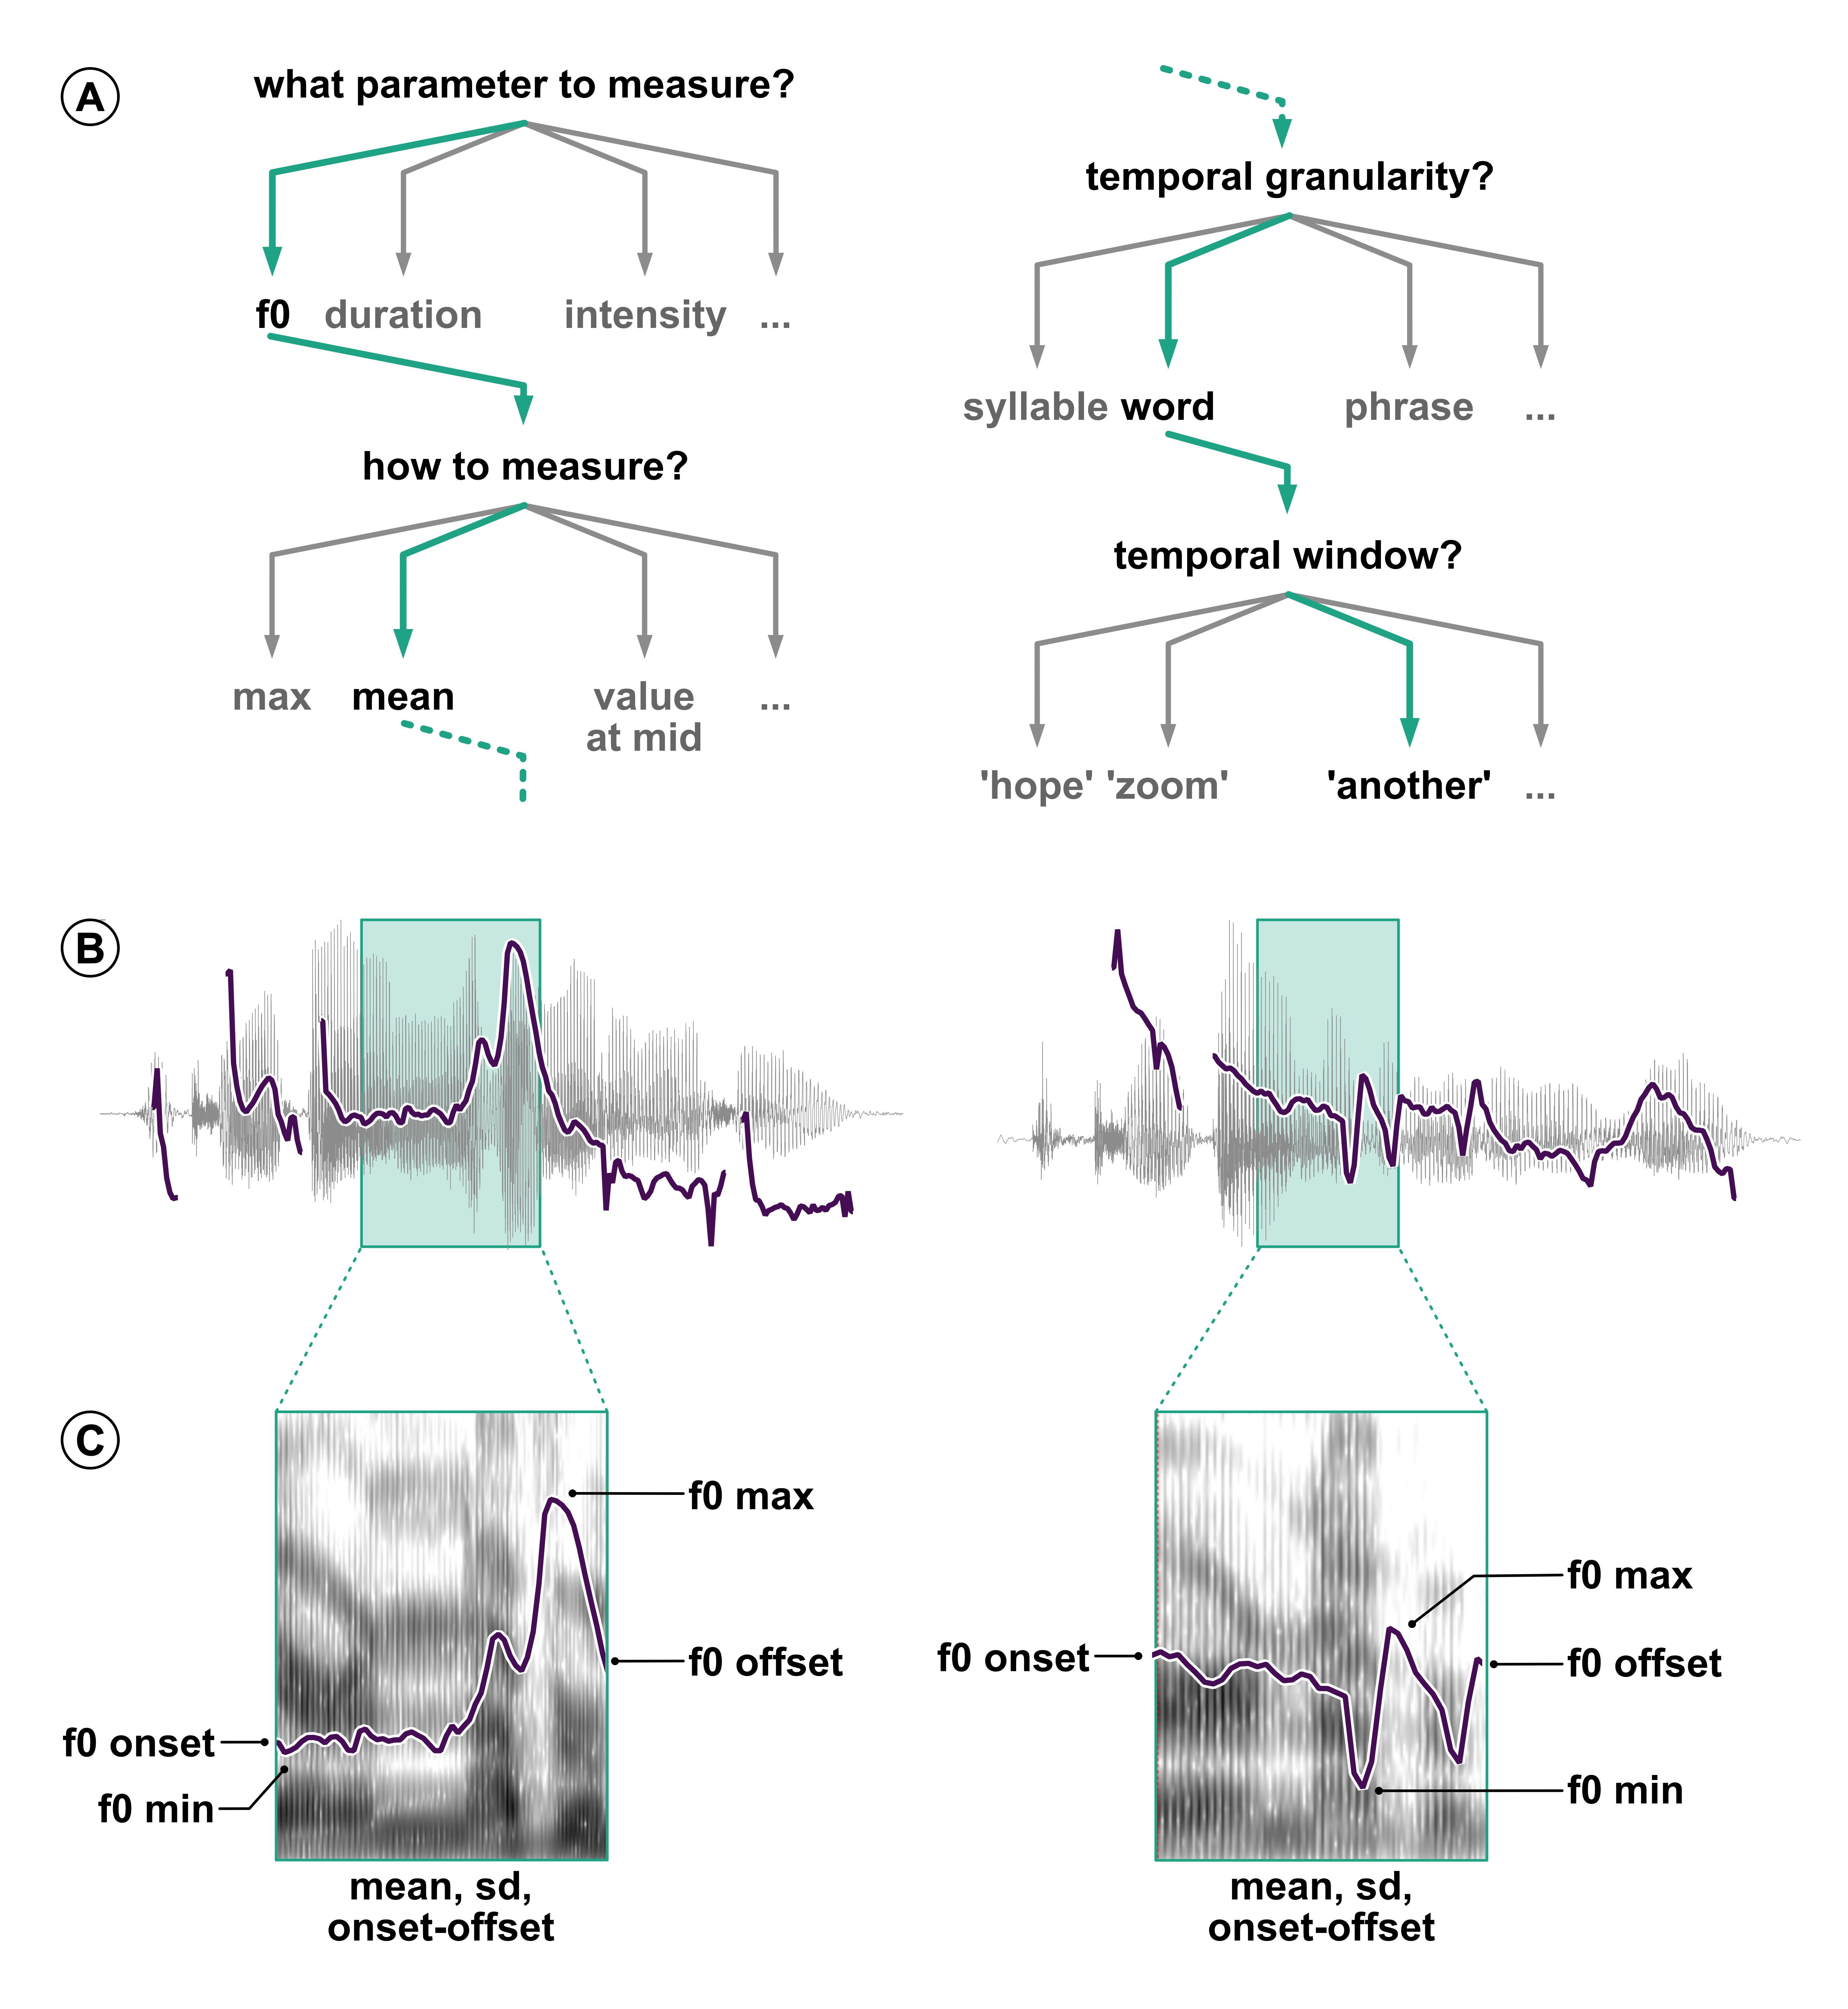
\includegraphics[width=1\linewidth]{../figs/ForkingPaths} \caption{Illustration of the analytic flexibility associated with acoustic analyses. (A) An example of multiple possible and justifiable decisions when comparing two utterances; (B) Waveform and f0 track of the utterances \emph{I can't bear ANOTHER meeting on Zoom} and \emph{I can't bear another meeting on ZOOM}. The green boxes mark the word \emph{another} in both sentences; (C) Spectrogram and f0 track of the word \emph{another}, exemplifying possible operationalizations of differences in f0.}\label{fig:forkingPaths}
\end{figure}

When looking at phrase-level temporal domains, the number of possible alternative analytic pipelines increases substantially.
Figure \ref{fig:forkingPaths}A shows a typical example of a decision tree with which speech researchers are often confronted.
Each of the four analytic decisions in the example have different possible options.
Here only one particular path has been taken. A different one would likely produce different results and might lead to different conclusions.
Once we have decided to compare f0 of the word \emph{another} across the two utterances, there are still many choices to be made, all of which need to be justified.
As Figures \ref{fig:forkingPaths}B-C illustrate, we could measure f0 at specific points in time like the onset of the temporal window, the offset, or the midpoint.
We could also measure the value or time of the f0 minimum or maximum.
We could summarize f0 across the entire window and extract the mean, median or standard deviation of f0, all of which have been used to analyze speech data in previous work \citep[see][]{gordon2017acoustic}.
But the journey in the garden of analytic paths goes on.
Other important operationalization steps could involve filtering the audio signal, smoothing the extracted f0 track, removing values that substantially deviate from surrounding values or expectations, either manually or automatically, and so on.

These decisions are intended to be made prior to any statistical analysis, but are at times revised \emph{a posteriori} in light of unforeseen or surprising outcomes (i.e.~after data collection and/or preliminary analyses).
This multitude of possible decisions are multiplied by those researcher degrees of freedom related to statistical analysis \citep[e.g.][]{wicherts2016}.

In sum, speech data is made of complex physical signals that generate an as-of-yet unappreciated amount of analytic flexibility in the choice of measures and operationalizations.
The present paper probes this garden of forking paths in the analysis of speech.
To assess the variability in data analysis pipelines, including both operationalization and statistical analysis, across independent researchers, we provide analytic teams with an experimentally elicited speech production data set.
The data set derives from the unpublished research project \emph{Prosodic encoding of redundant referring expressions}, which set out to investigate whether speakers acoustically modify utterances to signal unexpected referring expressions.\footnote{Results of this research project were neither published nor publicly presented and are stored on a private OSF repository.}
In the following section we introduce the research question and the experimental procedure of said project, and we describe the resulting data set as used in the current study.

\hypertarget{s:dataset}{%
\subsection{The data set: The acoustic properties of atypical modifiers}\label{s:dataset}}

Referring is one of the most basic and prevalent uses of language and one of the most widely researched areas in Language Science.
When trying to refer to a banana, what does a speaker say and how do they say it in a given context?
The context within which an entity occurs (i.e., with other non-fruits, other fruits, or other bananas) plays a large part in determining the choice of referring expressions.
Generally, speakers aim to be as informative as possible to uniquely establish reference to the intended object, but they are also resource-efficient in that they avoid redundancy \citep{grice1975logic}.
Thus one would expect the use of a modifier, for example, only if it is necessary for disambiguation.
For instance, one might use the adjective \emph{yellow} to describe a banana in a situation in which there are both a yellow and a less ripe green banana available, but not when there is only one banana.

Despite the coherent idea that speakers are both rational and efficient, there is much evidence that speakers are often over-informative.
Speakers use referring expressions that are more specific than strictly necessary for the unambiguous identification of the intended referent \citep{sedivy2003pragmatic, rubio2016redundant}, which has been argued to facilitate object identification and make communication between speakers and listeners more efficient \citep{arts2011overspecification, paraboni2007generating, rubio2016redundant}.
Recent findings suggest that the utility of referring expressions depends on how useful they are for a listener (compared to other referring expressions) to identify a target object.
For example, \citet{degen2020redundancy} showed that modifiers that are less typical for a given referent (e.g.~a blue banana) are more likely to be used in an over-informative scenario (e.g.~when there is just one banana)\citep[see also][]{westerbeek2015stored}.
This account, however, has mainly focused on content selection \citep{gatt2013we}, i.e.~what words to use.

Even when morphosyntactically identical expressions are involved, speakers can modulate utterances via acoustic properties like temporal and spectral modifications \citep[e.g.,][]{ladd2008intonational}.
Most prominently, languages can use intonation to signal discourse relationships between referents.
Intonation marks discourse-relevant referents for being new or given information, to guide the listeners' interpretation of incoming messages.
Beyond structuring information relative to the discourse, a few studies suggest that speakers might use intonation to signal atypical lexical combinations \citep[e.g.][]{dimitrova2008prosodic, dimitrova2009did}.
Referential expressions such as \emph{blue banana} were produced with greater prosodic prominence than more typical referents such as \emph{yellow banana}.
These results are in line with the idea of resource-efficient, rational language users who modulate their speech in order to facilitate listeners' comprehension.
However, the above studies are based on a small sample size (10 participants) and on potentially anti-conservative statistical analyses, leaving reason to doubt the generalizability of the studies' conclusions.

To further illuminate the question of whether speakers modify speech to signal atypical referents, and overcome some of the limitations of previous work, thirty native German speakers were recorded in a production study while interacting with a confederate (one of the experimenters) in a referential game, following experimental procedures typical of the field.
The participants had to verbally instruct the confederate to select a specified target object out of four objects presented on a screen.
The subject and confederate were seated at the opposite sides of a table, each facing one of two computer screens.
The participant and the experimenter could not see each other nor each others' screens.
Figure \ref{fig:procedural} shows the experimental procedure time-line.
After a familiarization phase, the subject first saw four colored objects in the top left, top right, bottom left, and bottom right corners of the screen.
One of the objects served as the target, another as the competitor, and the remaining two objects served as distractors.
Objects were referred to using noun phrases consisting of an adjective modifier denoting color and a modified object (e.g.~\emph{gelbe Zitrone} `yellow lemon', \emph{rote Gurke} `red cucumber', \emph{rote Socken} `red socks').



\begin{figure}
\includegraphics[width=1\linewidth]{../figs/procedure_plot} \caption{Experimental procedure. The upper row illustrates the trial sequence for the speaker (participant) and the lower row illustrates the trial sequence for the confederate. After a preview of 1500ms the speaker sees an arrow indicating one of the referents (b). Reading the orthographic instructions out loud, the speaker gives the confederate verbal instructions onto which referent they should drag the cube (c). The confederate, in turn, drags the black cube onto the target referent (d). Both the arrow and the orthographic instruction disappear from the speaker's screen and a new referent is indicated by an arrow on the same display alongside a new orthographic instruction (e). The speaker gives the confederate verbal instructions (f) which the confederate follows by dragging the cube onto the next referent (g).}\label{fig:procedural}
\end{figure}

In the center of the screen, a black cube was displayed, which could be moved by the experimenter.
Participant read a sentence prompt out loud (\emph{Du sollst den Würfel auf der COLOR OBJECT ablegen} `You have to put the cube on top of the COLOR OBJECT') to instruct the experimenter to drag the cube on top of one of the four depicted objects (the \emph{competitor}) using the mouse.
After the experimenter had moved the cube as instructed, the subject would read another sentence prompt (\emph{Und jetzt sollst du den Würfel auf der COLOR OBJECT ablegen} `And now, you have to put the cube on top of the COLOR OBJECT') instructing the experimenter to move the cube on top of a different object (the \emph{target}).
The second utterance in the trial was the critical trial for analysis.

The two sentence prompts were used to create a focus contrast between the competitor and the target object.
Focused units denote the set of all (contextually relevant) alternatives \citep[e.g.,][]{rooth1992theory}.
Concretely, a focus contrast marks one or more elements in a sentence as prominent, by different linguistic means depending on the language \citep{matic2013meanings, BURDIN2015254}.
For instance, if the competitor and target objects differ but their color does not (e.g.~\emph{yellow banana} vs.~\emph{yellow tomato}), the noun is said to be in focus (Noun Focus condition, NF).
If the objects are the same but differ in color (e.g.~\emph{yellow banana} vs.~\emph{blue banana}), the color adjective is in focus (Adjective Focus condition, AF).
If both the color and the object differ (e.g.~\emph{yellow banana} vs.~\emph{blue tomato}), then the whole noun phrase is in focus (Adjective/Noun Focus condition, ANF).
The NF condition constituted the experimentally relevant condition, while the AF and ANF conditions acted as fillers.
Crucially, the color-object combinations in the Noun Focus (NF) condition were manipulated with respect to their typicality.
The combinations were either typical (e.g.~\emph{orange mandarin}), medium typical (e.g.~\emph{green tomato}), or atypical (e.g.~\emph{yellow cherry}), as established by a norming study that was conducted prior to the production experiment just described.\footnote{A detailed description of the norming and production studies from the \emph{Prosodic encoding of redundant referring expressions} project, which was given to the analysts with the data set, can be found in \texttt{methods\_norm\_prod.pdf} at \url{https://bit.ly/3Ahawc7}.}
Each subject produced 15 critical trials (NF condition).
Each trial was repeated twice, yielding a total of 30 trials per participant and a grand-total of 900 (\(15 \times 2 \times 30\) participants) spoken utterances.

For the present study, 46 analysis teams have received access to the entire data set generated by the production study.
The data set is constituted by audio recordings and annotation files in a format that is typical for the field.
The teams were instructed to answer the following research question, using the provided data set: \emph{Do speakers acoustically modify utterances to signal atypical word combinations?}

\hypertarget{methods}{%
\section{Methods}\label{methods}}

As outlined in Section \protect\hyperlink{s:operspeech}{Operationalizing speech}, researchers are faced with a large number of analytic choices when analyzing a multidimensional signal such as speech.
Analysts must identify and operationalize relevant measurements, as well as the temporal domain(s) from which these measurements are to be taken, and then possibly transform said measurements before submitting them to statistical models, which must be chosen alongside inferential criteria.
The complexity of speech data constitutes the ideal testing ground to assess the upper bound of analytic flexibility that social science might face across disciplines.
We employed a meta-analytic approach to assess (i) the variability of the reported effects, and (ii) how analytic and researcher-related predictors affect the final results.

In this study, we followed the procedures proposed by \citet{Parker2020} and \citet{aczel2021}.
The project comprised the following five phases:

\begin{enumerate}
\def\labelenumi{\arabic{enumi}.}
\tightlist
\item
  \textsc{Recruitment}: We recruited independent groups of researchers to analyze the data and review others' data analyses.
\item
  \textsc{Team Analysis}: We gave researchers access to the speech corpus and let them analyze the data as they saw fit.
\item
  \textsc{Review}: We asked reviewers to generate peer-review ratings of the analyses based on methods (not results).
\item
  \textsc{Meta-analysis}: We evaluated variability among the different analyses and how different predictors affected the outcomes.
\item
  \textsc{Write-up}: We collaboratively produced the final manuscript.
\end{enumerate}

We initially estimated that this process, from the time of an in-principle acceptance of the Stage 1 Registered Report to the end of Phase 5, would take nine months.
Phase 4 (meta-analysis) took longer than initially anticipated and the total duration of the project was approximately 12 months.

The project OSF repository contains all the materials mentioned in this paper and can be accessed at \url{https://osf.io/3bmcp/}.
The repository holds three main OSF components (\texttt{Data}, \texttt{Teams\ analyses} and \texttt{Questionnaires}), and a link to the project's GitHub repository.
The following sections report the criteria for sample size, data exclusions, data manipulations, and all the measures in the study.

\hypertarget{phase-1-recruitment-of-analysts-and-initial-survey}{%
\subsection{Phase 1: Recruitment of analysts and initial survey}\label{phase-1-recruitment-of-analysts-and-initial-survey}}

An online landing page provided a general description of the project, including a short pre-recorded slide-show that summarizes the data set and research question (\url{https://many-speech-analyses.github.io}).
The project was advertised via social media, using mailing lists for linguistic and psychological societies, and via word of mouth.
Social media advertising was accompanied by a short recruitment form (\texttt{recruitment\_form.pdf}).
The target population comprised active speech science researchers with a graduate/doctoral degree (or currently studying for a graduate/doctoral degree) in relevant disciplines.
All individuals interested in participating were asked to complete a questionnaire detailing their familiarity with numerous analytic approaches common in the speech sciences (\texttt{analytic\_approach\_quest.pdf}).
Researchers could choose to work independently or in small teams.
For the sake of simplicity, we will refer both to a single researcher and teams as \textsc{analysis teams}.\footnote{Terms in small caps in this and later sections are included with their definition in the glossary at the end of the paper for the reader's convenience.}
Recruitment for this project commenced after having received in-principle acceptance.

As outlined above, our primary aim is to assess the variability of the reported effects, rather than the meta-analytic estimate of the investigated effect \emph{per se}.
To estimate the degree of uncertainty around effect variability as driven by number of teams, we ran a series of sample size simulations with values of variability extracted from \citet{silberzahn2018many}.
The code is available at \url{https://many-speech-analyses.github.io/many_analyses/scripts/r/simulations/simulations}, Section 2.\footnote{Cached model outputs can be found at \url{https://osf.io/wds2m/}.}
Variability among teams was operationalized as the standard deviation of the teams' reported effects from \citet{silberzahn2018many} (which we \emph{z}-scored prior to simulations to make it comparable to our study).
For the mean of the teams' true standard deviation (0.68 \emph{z}-score), the simulation indicates that the degree of uncertainty around the estimated teams' standard deviation will be below 1 SD at any sample size greater than 10 teams.
Thus in order to achieve our main goal, i.e.~estimating variability among teams, we considered a minimum sample size of 10 teams as sufficient.
Given the exploratory nature of our study, however, we have sampled as many analysts as possible.
We received initial expressions of interest to participate from more than 200 analysts, though there was a substantial drop-out rate (see Section Results).

After submitting their analyses, we asked the analysts to also function as peer-reviewers.
Each team had to review four other analyses.
All analysts involved share co-authorship on this manuscript and participated in the collaborative process of producing the final manuscript.
Informed consent was obtained as part of the intake form.

\hypertarget{phase-2-primary-data-analyses}{%
\subsection{Phase 2: Primary Data Analyses}\label{phase-2-primary-data-analyses}}

The analysis teams registered for participation and each of the analysts individually answered a demographic and expertise questionnaire (\texttt{intake\_form.pdf}).
A PDF version of this and all other questionnaires are available in the repository's \texttt{Questionnaires} component, at \url{https://osf.io/h6z8w/}.
The questionnaire collected information on the analysts' current position and self-estimated breadth and level of statistical expertise and acoustic analysis skills.
We then requested that they answer the research question: \emph{Do speakers acoustically modify utterances to signal atypical word combinations?}
To do so, they were given the data generated by the experiment described in Section \protect\hyperlink{s:dataset}{The data set}.
Data included the audio recordings with corresponding time-aligned transcriptions in the form of Praat TextGrid files.
These can be found in the \texttt{Data} component at \url{https://osf.io/5agn9/}.

Once their analysis was complete, they answered a structured questionnaire (\texttt{analytic\_quest.pdf}), providing information about their analysis technique, an explanation of their analytic choices, their quantitative results, and a statement describing their conclusions.
They also uploaded their analysis files (including the additionally derived data and text files that were used to extract and pre-process the acoustic data), their analysis code (if applicable), and a detailed journal-ready analysis section.

\hypertarget{phase-3-peer-review-of-analyses}{%
\subsection{Phase 3: Peer Review of Analyses}\label{phase-3-peer-review-of-analyses}}

The analyses from each team were evaluated by four different teams who functioned as peer-reviewers.
Each peer-reviewer was randomly assigned to analyses from at least four analysis teams.
Reviewers evaluated the methods of each of their assigned analyses one at a time in a sequence determined by the initiating authors.
The sequences were systematically assigned so that, if possible, each analysis is allocated to each position in the sequence for at least one reviewer.

The process for a single reviewer was as follows.
First, the reviewer received a description of the methods of a single analysis.
This included the narrative methods and results sections, the analysis team's answers to the questionnaire regarding their methods, including analysis code and the data set.
The reviewer was then asked in an online questionnaire (\texttt{peer\_review\_quest.pdf}) to rate both the acoustic and the statistical analyses and to provide an overall rating, using a scale of 0-100, respectively.
To help reviewers calibrate their rating, they were given the following guidelines:

\begin{itemize}
\item
  \begin{enumerate}
  \def\labelenumi{\arabic{enumi}.}
  \setcounter{enumi}{99}
  \tightlist
  \item
    A perfect analysis with no conceivable improvements from the reviewer.
  \end{enumerate}
\item
  \begin{enumerate}
  \def\labelenumi{\arabic{enumi}.}
  \setcounter{enumi}{74}
  \tightlist
  \item
    An imperfect analysis but the needed changes are unlikely to dramatically alter the final interpretation.
  \end{enumerate}
\item
  \begin{enumerate}
  \def\labelenumi{\arabic{enumi}.}
  \setcounter{enumi}{49}
  \tightlist
  \item
    A flawed analysis likely to produce either an unreliable estimate of the relationship or an over-precise estimate of uncertainty.
  \end{enumerate}
\item
  \begin{enumerate}
  \def\labelenumi{\arabic{enumi}.}
  \setcounter{enumi}{24}
  \tightlist
  \item
    A flawed analysis likely to produce an unreliable estimate of the relationship and an over-precise estimate of uncertainty.
  \end{enumerate}
\item
  \begin{enumerate}
  \def\labelenumi{\arabic{enumi}.}
  \setcounter{enumi}{-1}
  \tightlist
  \item
    A dangerously misleading analysis, certain to produce both an estimate that is wrong and a substantially over-precise estimate of uncertainty that places undue confidence in the incorrect estimate.
  \end{enumerate}
\end{itemize}

\noindent The reviewers were also given the option to include further comments in a text box for each of the three ratings.

After submitting the review, a methods section from a second analysis was made available to the reviewer.
This same sequence was followed until all analyses allocated to a given reviewer were provided and reviewed.\footnote{Initially we planned to present simultaneously all four (or more) methods sections to each reviewer after the fourth round, with the option to revise their original ratings and provide an explanation. Ultimately, we decided to skip this step due to time constraints.}

\hypertarget{phase-4-evaluating-variation}{%
\subsection{Phase 4: Evaluating variation}\label{phase-4-evaluating-variation}}

The initiating authors (SC, JC, TR) conducted the analyses outlined in this section.
We did not conduct confirmatory tests of any \emph{a priori} hypotheses.
We consider our analyses exploratory.

\hypertarget{descriptive-statistics}{%
\subsubsection{Descriptive statistics}\label{descriptive-statistics}}

We calculated summary statistics describing variation among analyses, including (a) the nature and number of acoustic measures (e.g.~f0 or duration), (b) the operationalization and the temporal domain of measurement (e.g.~mean of an interval or value at a specified point in time), (c) the nature and number of model parameters for both fixed and random effects (if applicable), (d) the nature and reasoning behind inferential assessments (e.g.~dichotomous decision based on \emph{p}-values, ordinal decision based on a Bayes factor), as well as the (e) mean, (f) standard deviation and (g) range of the standardized effect sizes (see the next section for the standardization procedure).
These summary statistics are reported in \emph{Descriptive statistics} of the Results section.

\hypertarget{meta-analytic-estimation}{%
\subsubsection{Meta-analytic estimation}\label{meta-analytic-estimation}}

We investigated the variability in \textsc{reported effect sizes} using Bayesian meta-analytic techniques.
As the measure of variability, we took the meta-analytic \textsc{group-level standard deviation} (\(\sigma_{\alpha_{\text{t}}}\), see below), where each analysis team represents a group.
As we detail in the Results section below, we have also run further non-preregistered analyses.
For these we refer the reader to that section, while we only describe the preregistered analyses in the following paragraphs.

Based on the common practices currently in place within the field, we anticipated that researchers would use multilevel regression models, thus common measurements of effect size, such as Cohen's \(d\), might have been inappropriate.
Furthermore, \citet{aczel2021} suggest that directly asking analysts to report standardized effect sizes could bias the choice of analyses towards types that more straightforwardly return a standardized effect.
Since the variables used by the analysis teams might have substantially differed in their measurement scales (e.g, Hertz for frequency vs.~milliseconds for duration) which was indeed the case, we have standardized all reported effects by refitting each \textsc{reported model} with centered and scaled continuous variables (\emph{z}-scores, i.e.~the observed values subtracted from the mean divided by the standard deviation) and sum-coded factor variables.
Each \textsc{standardized model} was fitted as a Bayesian regression model with Stan \citep{stan2021}, RStan \citep{stan2020a}, and brms \citep{burkner2017} in R \citep{R-base}.
Model refitting also constituted a way of validating the reported analyses, a step recommended by \citet{aczel2021}.
Details about the refitting procedure can be found at \url{https://many-speech-analyses.github.io/many_analyses/scripts/r/04_refit_workflow}.
Relative to the registered protocol, we made minor changes to the refitting procedure, specifically file and variable naming conventions and the use of treatment contrasts instead of sum coding.
All models converged (\(\hat{R}\) was approximately 1).
Of the models with divergent transitions (n = 10), the number of divergences ranged from 1 to 156 (143 represents 3.9\% of total number of samples), which the authors deemed not to be problematic.

The coefficients of the critical predictors (i.e.~critical according to the analysis teams' self-reported inferential criteria) obtained from the standardized models were used as the \textsc{standardized effect size} (\(\eta_i\)) of each reported model.
Moreover, to account for the differing degree of uncertainty around each standardized effect size, we used the standard deviation of each standardized effect size as the \textsc{standardized standard error} (\(\text{se}_i\)).
This enabled us to fit a so-called ``measurement-error'' model, in which both the standardized effect sizes and their respective standard errors are entered in the meta-analytic model.
As a desired consequence, effect sizes with a greater standard error are weighted less than those with a smaller standard error in the meta-analytic calculations.

After having obtained the standardized effect sizes \(\eta_i\) with related standard errors \(\text{se}_i\), for each critical predictor in each reported model, we conducted a \textsc{Bayesian random-effects meta-analysis} using a multi-level (intercept-only) regression model.
The outcome variable was the set of standardized effect sizes \(\eta_i\).
The likelihood of \(\eta_i\) was assumed to correspond to a normal distribution \citep{knight2000}.
The analysis teams were entered as a group-level effect (i.e., \texttt{(1\ \textbar{}\ team)}, called \emph{random effect} in the frequentist literature).
The standard errors \(\text{se}_i\) were included as the standard deviation of \(\eta_i\) to fit a measurement-error model, as discussed above.
We used regularizing weakly-informative priors for the intercept \(\alpha\) (\(Normal(0, 1)\)) and for the group-level standard deviation \(\sigma_{\alpha_{\text{t}}}\) (\(HalfCauchy(0, 1)\)).
We fit this model with 4 chains of Hamiltonian Monte-Carlo sampling for the estimation of the joint posterior distribution, using the No U-Turn Sampler (NUTS) as implemented in Stan \citep{stan2021}, and 4000 iterations (2000 for warm-up) per chain, distributed across 8 processing cores and 2 threads in within-chain parallelization.
The model did not incur any divergent transitions (\(\hat{R}\) was not greater than 1) and the estimated sample sizes were sufficient.
The code used to run the model can be found at \url{https://many-speech-analyses.github.io/many_analyses/scripts/r/06_meta-analysis_prereg}.

The posterior distribution of the population-level intercept \(\alpha\) allowed us to estimate the range of probable values of the standardized effect size \(\hat{\eta}\).
The posterior distribution further allowed us to investigate the effect of a set of analytic and researcher-related predictors, detailed in the next section.
Crucially, the posterior distribution of the \href{.smallcaps}{group-level standard deviation} \(\sigma_{\alpha_{\text{t}}}\) (i.e.~the standard deviation of the group-level effect of team) allowed us to quantify the degree of variation between the teams' analyses on a standardized scale.

\hypertarget{anares-preds}{%
\subsubsection{Analytic and researcher-related predictors affecting effect sizes}\label{anares-preds}}

As a second step, we investigated the extent to which the individual standardized effect sizes are affected by a series of \textsc{analytic and researcher-related predictors}.

\textbf{Analytic predictors}. We estimated the influence of the following predictors related to the analytic characteristics of each team's reported analysis:

\begin{itemize}
\tightlist
\item
  \emph{Measure of uniqueness} of individual analyses for the set of predictors in each model {[}numeric{]}.
\item
  \emph{Number of models} the teams reported to have run {[}numeric{]}.
\item
  \emph{Major dimension} that has been measured to answer the research question {[}categorical{]}.
\item
  \emph{Temporal window} that the measurement is taken over {[}categorical{]}.
\item
  \emph{Average peer-review rating}, as the mean of the overall peer-review ratings for each analysis {[}numeric{]}.
\end{itemize}

Following \citet{Parker2020}, the measure of uniqueness of predictors was assessed by the Sørensen-Dice Index \citep[SDI,][]{dice1945, sorensen1948}.
The SDI is an index typically used in ecology research to compare species composition across sites.
It is a distance measure similar to Euclidean distance measures, but is more sensitive to more heterogeneous data sets and deemphesizes outliers.
For our purposes, we treated predictors as \emph{species} and individual analyses as \emph{sites}.
For each pair of analyses \((X, Y)\) (across and within teams), the SDI was obtained using the following formula:

\[\text{SDI} = \frac{2|X \cap Y|}{|X|+|Y|}\]
\vspace{0.05in}

\noindent where \(|X \cap Y|\) is the number of variables common to both models in the pair, and \(|X|+|Y|\) is the sum of the number of variables that occur in each model.
For example, if two pairs of models differ in either only one predictor (e.g.~DV \textasciitilde{} typicality vs.~DV \textasciitilde{} typicality + trial) or in two predictors (e.g.~DV \textasciitilde{} typicality vs.~DV \textasciitilde{} typicality + trial + speech rate), the latter model pair would exhibit a larger SDI than the former.
In order to generate a unique SDI for each analysis team, we calculated the average of all pairwise SDIs for all pairs of analyses using the \texttt{beta.pair()} function in the betapart R package \citep{baselga2020}.

The major measurement dimension of each analysis was categorized according to the following possible groups: \emph{duration}, \emph{intensity}, \emph{f0}, \emph{other spectral properties} (e.g.~frequency, center of gravity, harmonics difference, etc.), and \emph{other measures} (e.g.~derived measures such principal components, vowel dispersion, etc.).
The temporal window that the measurement is taken over is defined by the target linguistic unit.
We assume the following relevant linguistic units: \emph{segment}, \emph{syllable}, \emph{word}, \emph{phrase}, \emph{sentence}.
Since each analysis received more than one peer-review rating, we calculated the mean rating and its standard deviation for each.
These were entered in the model formula as a measurement-error term (\texttt{me(mean,\ sd)} in brms).

\textbf{Researcher-related factors}. We also included the following predictors:

\begin{itemize}
\tightlist
\item
  \emph{Research experience} as the elapsed time from receiving the PhD. Negative values will indicate that the person is a student or graduate student {[}numeric{]}.
\item
  \emph{Initial belief} in the presence of an effect of atypical noun-adjective pairs on acoustics, as answered during the intake questionnaire {[}numeric{]}.
\end{itemize}

To obtain an aggregated research experience score and initial belief score for each team based on the members' individual scores, we calculated the mean and standard deviation of these predictors for each team.
These were entered in the model formula as a measurement-error term (\texttt{me(mean,\ sd)} in brms).
The expedient of using a measurement-error term (which includes the teams' standard deviation) ensures information about within-team variance is not lost (which would be the case if including the mean only).

We had initially planned to also include a measure of conservativeness of the model specification, as the number of random/group-level effects included and the number of post-hoc changes to the acoustic measurements the teams reported to have carried out.
When fitting the model, we realized that the measure of conservativeness is related to the standard error of the estimates (i.e.~more group-level effects = higher standard error).
Moreover, there was no team that declared to have made post-hoc changes to the analyses, thus we decided against including these two preregistered predictors in the model.

\textbf{Model specification}. The model was fitted as a measurement-error model, with the predictors detailed in the preceding paragraphs.
The outcome variables of the model were the standardized effect sizes and related standard deviation.

A normal distribution was used as the likelihood function of \(\alpha_{t[i]}\).
The mean of \(\alpha_{t[i]}\) was modeled on the basis of the overall intercept \(\beta\) and on the coefficients of each predictor.
The numeric predictors were centered and scaled and the categorical predictors were sum coded.
We used a normal distribution with mean 0 and standard deviation 1 as the prior for the intercept and the predictors.
The model was run with the same settings as with the meta-analytic model.
The code used to run the model can be found at \url{https://many-speech-analyses.github.io/many_analyses/scripts/r/06_meta-analysis_prereg}.

\hypertarget{ana-archive}{%
\subsubsection{Data management}\label{ana-archive}}

All relevant data, code, and materials have been publicly archived on the Open Science Framework (\url{https://osf.io/3bmcp/}).
Archived data include the original data set distributed to all analysts, any edited versions of the data analyzed by individual teams, and the data we analyzed with our meta-analyses, which include the standardized effect sizes, the statistics describing variation in model structure among analysis teams, and the anonymized answers to our questionnaires of analysts.
Similarly, we archived both the analysis code used for each individual analysis and the code from our meta-analyses.
We also archived copies of our survey instruments from analysts and peer-reviewers.
Further documents concerning the collaborative editing of the Registered Report can be found at \url{https://drive.google.com/drive/folders/1-DOcj1qtEkvWfzu_FrsxkIGfPS0DyLXB?usp=sharing}.

We excluded from our synthesis any individual analysis submitted after peer review (Phase 3) or those unaccompanied by analysis files without which it was not possible to follow the research protocol.
We also excluded any individual analysis that does not produce an outcome that could be interpreted as an answer to our primary question.
We also did no include analyses for which we could not extract standardized effect sizes. For a list of exclusion criteria, see Section Descriptive statistics below.

\hypertarget{phase-5-collaborative-write-up-of-manuscript}{%
\subsection{Phase 5: Collaborative Write-Up of Manuscript}\label{phase-5-collaborative-write-up-of-manuscript}}

The initiating authors discussed the limitations, results, and implications of the study and collaborated with the analysts on writing the final manuscript for review as a stage-2 Registered Report.\footnote{The comment history can be found at \url{https://docs.google.com/document/d/1CFgRo93mRgifpuFOuQE3vNBeMW-H7ps9eD--vxH-6CQ/edit?usp=sharing}.}

\hypertarget{results}{%
\section{Results}\label{results}}

The results section is divided into three parts.
We first provide a statistical description of team composition, nature of acoustic analyses and statistical approaches, and peer-review ratings.
Second, we report the results of the meta-analytic model, focusing on between-team and between-model variability.
Finally, we present the analysis of the effect of analytic and researcher-related predictors on the meta-analytic effect.
The research compendium of the study, containing all the code and data presented here, can be found in the GitHub repository linked in the research compendium at \url{https://osf.io/3bmcp/}, in the \texttt{scripts/r/} folder.
An interactive web application that allows the interested reader to explore the data set is available at \url{https://many-speech-analyses.github.io/shiny}.

\hypertarget{descr-stats}{%
\subsection{Descriptive statistics}\label{descr-stats}}

In the following sections, we will describe the characteristics of the analysis teams that participated in the study and the analytic approaches they adopted.
An important aspect that emerges from the descriptive analysis is the large variation in analytic strategies.

\hypertarget{characteristics-of-analysis-teams}{%
\subsubsection{Characteristics of analysis teams}\label{characteristics-of-analysis-teams}}

Eighty-four teams initially signed up to participate in the study, comprising 211 analysts.
Thirty-eight of the signed-up teams dropped out during the analysis phase.

Forty-six teams submitted their analyses by the established deadline.
Only analyses from which it was possible to extract an effect size were included in the meta-analysis.
Of the analyses submitted by the 46 teams, the initiating authors identified 33 teams with submissions meeting the criteria for inclusion in the meta-analytic model.
Reasons for exclusion were: use of Generalized Additive Models (4 teams) which do not lend themselves easily to the meta-analytic methods employed in this study, use of machine learning techniques (3 teams), use of typicality as the outcome variable/response (3 teams), or use of other methods that returned statistics that could not be included in the meta-analytic model.
Note that due to the unforeseen variability across teams, the latter exclusion criteria were not preregistered and were applied after having seen all analytic strategies.

In what follows, we describe the characteristics of those teams whose analyses were included in the meta-analytic model.
A complete summary of all the analyses from the 46 submitting teams is available in the supplementary materials at \url{https://many-speech-analyses.github.io/many_analyses/RR_manuscript/supplementary_materials.pdf}.

The included analyses were provided by 33 teams, comprising 120 analysts, with a median of 3.0 individuals per team.
Upon sign-up, we collected background information from each analyst through the intake form, which was administered during Phase 1, prior to the data being released to the teams.
Analysts had a median of 5.4 years of experience after completing their PhD, ranging from -3.8 years, i.e.~PhD students (or less experienced) to 12.4 years, suggesting that, on average, analysts were experienced researchers.
The analysts' prior belief in the effect under investigation, on a scale from 0 to 100, ranged from 46.4 to 92.0 with a median of 70.0.
We take this to suggest that, overall, analysts had a rather high positive prior belief in the investigated relationship between acoustics and word combination typicality.

At the end of Phase 2 (primary data analysis), the teams had submitted a grand total of 115 individual models (including 192 critical model coefficients, given that some models returned more than one critical coefficient) to answer the research question, with a median of 3 models per team.
Table \ref{tab:descriptives-table} provides a summary of the contributing teams and their analyses.

\hypertarget{acoustic-analysis}{%
\subsubsection{Acoustic analysis}\label{acoustic-analysis}}

The analytic teams differed in their approach to the acoustic analysis of the speech signal, including choices related to specific acoustic measures, the temporal window used, and how the measures were transformed.
Thirty-seven percent of the models used f0 as the outcome variable, 33\% used a measure of duration, 13\% used vowel formants, 15\% intensity, and 3\% other measures.

Forty-five percent of models used acoustic measures taken at the level of the segment (e.g.~comparing the acoustic profile of a vowel), 45\% from the word level (e.g.~comparing the acoustic profile of \emph{Banane} `banana'), 3\% at the level of the phrase (e.g.~the noun phrase including determiner and adjective, e.g.~``the green banana''), 3\% from the whole sentence, and 3\% used a different time window.
Based on a coarse coding of how acoustic measures were operationalized, we find a total of 55 different measurement specifications.
For example, if we consider those analyses that target f0, we find that it is operationalized in many different ways including the minimum, the maximum, the mean, the median, as a range in an interval or a ratio between two intervals.
The measurement is sometimes taken from the interval of a vowel in the article, the adjective or noun; it is sometimes taken from the word interval of the article, adjective or noun; or it is taken from either the noun phrase interval or the entire sentence.
Some of these measures were normalized relative to other elements in the sentence or relative to the speaker.

\hypertarget{statistical-analysis}{%
\subsubsection{Statistical analysis}\label{statistical-analysis}}

The large decision space related to how the acoustic signal was measured is further expanded by the choices in the statistical analysis, including the chosen inferential framework, the type of model, and the model specification, including choice of predictors, interactions and group-level effects.

The mean of the number of different predictors included in teams' models was 2 (defined as variables or columns in the data table).
This means that, in addition to the critical predictor (typicality of the adjective noun combinations), models had on average one additional predictor (range = 1 - 5).
Possible information that was used as predictors included the information structure of the sentence, trial number, semantic dimensions of the referent, part of speech, and speaker gender.

The data given to the teams allowed them to operationalize the predictor of interest, word typicality, in different ways.
Among the possible operationalizations, 69\% of models contained typicality as a categorical variable (e.g.~atypical vs.~typical), 28\% used a continuous typicality scale from 0-100 by calculating the mean typicality for each word combination as obtained from the norming study, while 3\% of the models used the median typicality rating.
Note that the design of the experiment alongside its description indicated that the experiment was designed to categorically operationalize typicality. This possibly explains the analysts' strong preference.

The majority of models were run within a frequentist framework (84\%).
Sixteen percent were run within a Bayesian framework.
While teams almost exclusively used linear models to analyze their data (98\%), teams differed drastically in how they accounted for dependencies within the data.

The data contains several dependencies between data points, with multiple data points coming from the same subject and with multiple data points being associated with the same adjective or noun.
An appropriate way to account for this non-independence is by using models that include so-called random or group level effects \citep[e.g.,][]{gelman2006data, schielzeth2009conclusions}, variably known as mixed-effects, hierarchical, multi-level, or nested models (among other names).
Nine percent of the linear models specified no random effects at all (without pooling their data), effectively ignoring these non-independences \citep{hurlbert1984pseudoreplication}.
Sixty-two percent specified random intercepts only, and 29\% specified both random intercepts and random slopes to account for the non-independence.
On average, teams that specified random effects included 2.5 random terms in their models.
Based on statistical framework, type of model, distribution family, fixed terms, and not including random effects, there were a total of 52 different model specifications.

When considering both acoustic and statistical analyses, we have found a grand total of 119 different analytic pipelines.
In other words, each individual analysis submitted was unique.
A sankey diagram illustrating the relationship between choices related to outcome, temporal window and operationalization can be found in the supplementary materials at \url{https://many-speech-analyses.github.io/many_analyses/RR_manuscript/supplementary_materials.pdf}.

Our quantitative assessment did not include other degrees of freedom, all of which are additional sources of variation:
Teams differed with regard to how the acoustic signal was segmented ranging from fully automated forced-alignment with minimal manual correction to complete manual alignment performed by the analysts; teams differed in whether the statistical analysis was based on a subset of the data or the whole data set; and they differed whether and if so how measurements were excluded based on both qualitative (i.e.~whether specific speech production instances were excluded or not) and quantitative grounds (i.e.~whether data were trimmed or not).

The question arises whether these unique analysis pipelines led to different conclusions.
Thirteen teams out of the thirty-three (39.4\%) reported to have found at least one statistically reliable effect (based on the inferential criteria they specified).
Of the 192 critical model coefficients, 45 were claimed to show a statistically reliable effect (23.4\%).

\begin{table}

\caption{\label{tab:descriptives-table}Descriptive statistics of teams, acoustic analyses, and statistical analyses included in the meta-analysis. The data set included analyses from 33 teams and  120 analysts.}
\centering
\resizebox{\linewidth}{!}{
\begin{tabular}[t]{llrr}
\toprule
\bf{Team characteristics} &    & \bf{Range} & \bf{Median}\\
\midrule
 & Team size & 1.0 -- 12.0 & 3.0\\
 & Years after PhD & -3.8 -- 12.4 & 5.4\\
 & Prior belief & 46.4 -- 92.0 & 70.0\\
 & Acoustic analysis peer rating & 41.2 -- 88.3 & 73.8\\
 & Statistical analysis peer rating & 33.0 -- 93.3 & 73.2\\
 & Overall peer rating & 39.0 -- 88.7 & 70.8\\
 &  &  \vphantom{5} & \\
\bf{Acoustic analyses} &  & \bf{n} & \bf{\%}\\
\midrule
\hspace{1em}Outcome & F0 & 44 & 37\\
 & Duration & 39 & 33\\
 & Intensity & 18 & 15\\
 & Formants & 15 & 13\\
 & Other & 3 & 3\\
 &  &  \vphantom{4} & \\
\hspace{1em}Temporal window & Segment & 54 & 46\\
 & Word & 53 & 45\\
 & Sentence & 4 & 3\\
 & Phrase & 3 & 3\\
 & Other & 4 & 3\\
 &  &  \vphantom{3} & \\
\hspace{1em}Typicality operationalization & Categorical & 82 & 69\\
 & Continuous (mean) & 33 & 28\\
 & Continuous (median) & 3 & 3\\
 &  &  \vphantom{2} & \\
\bf{Statistical analyses} &  & \bf{n} & \bf{\%}\\
\midrule
\hspace{1em}Framework & Frequentist & 100 & 84\\
 & Bayesian & 19 & 16\\
 &  &  \vphantom{1} & \\
\hspace{1em}Model & Linear model & 117 & 98\\
 & GAM & 1 & 1\\
 & Other & 1 & 1\\
 &  &  & \\
 &  & \bf{Range} & \bf{Median}\\
\hspace{1em}N & Models & 1 -- 16 & 3\\
 & Predictors & 1 -- 5 & 2\\
 & Random terms & 1 -- 10 & 2\\
\hspace{1em} & \hspace{1em}Intercept & \hspace{1em}1 -- 10 & \hspace{1em}2\\
\hspace{1em} & \hspace{1em}Slope & \hspace{1em}0 -- 4 & \hspace{1em}0\\
\bottomrule
\end{tabular}}
\end{table}

\hypertarget{review-ratings}{%
\subsubsection{Review ratings}\label{review-ratings}}

Teams reviewed each others' acoustic and statistical analyses.
The mean rating of the acoustic analyses, on a scale from 0 to 100, is 71.5 (SD = 13.5).
The mean rating of the statistical analysis is 69.4 (SD = 15.9).
For reference, as mentioned in the Methods section, a score of 75 was defined as ``an imperfect analysis but the needed changes are unlikely to dramatically alter the final interpretation'', indicating that on average reviewers judged the provided analyses to be appropriate, although ``imperfect''.

\hypertarget{meta-est-2}{%
\subsection{Meta-analytic estimation}\label{meta-est-2}}

This section deals with the meta-analytic analysis of the results submitted by the teams.
As discussed above, the analyses of only 30 teams out of all the submitted analysis were included in the meta-analytic model discussed here.
First, we report on the between-team variability estimate (i.e.~the meta-analytic group-level standard deviation \(\sigma_{\alpha_{\text{t}}}\)), which is the focus of this study, followed by the meta-analytic estimate (i.e.~the intercept of the meta-analytic model, in other words, the estimated effect of typicality on the acoustic production of adjective-noun combinations).

\hypertarget{between-team-variability}{%
\subsubsection{Between-team variability}\label{between-team-variability}}

The primary aim of this analysis is to assess the degree of between-team variability.
As a measure of between-team variability, we chose to use the meta-analytic group-level standard deviation (\(\sigma_{\alpha_{\text{t}}}\)).

According to the preregistered meta-analytic model, the group-level standard deviation for teams is between 0.03 and 0.07 standard units at 95\% credibility.
In other words, the estimated range of variation across teams lies somewhere between \(\pm 0.06\) (0.03 * 1.96) and \(\pm 0.13\) (0.07 * 1.96) standard units with 95\% credibility.

\textbf{Non-preregistered}. However, in our preregistration we did not take into account that teams might submit multiple analyses/models which, if unaccounted for, violates the independence assumption.
Teams were explicitly instructed to only submit one effect size without enforcing it.
As a result, some teams followed the instruction and submitted only one model while others submitted multiple models.
To account for this added layer of dependency, we have run a model with team and model ID nested within team as group-level effects (\texttt{(1\textbar{}team)\ +\ (1\textbar{}team:model\_id)}), which allows us to estimate both the between-team variation and the between-analysis variation.
This analysis was not preregistered and should thus be interpreted with caution.\footnote{Note that before fitting this model, we fitted a separate one in which model ID was the only (non-nested) group-level effect.
  The estimated group-level effect of model ID is identical to that of the nested model, so we will not discuss it further.}

The nested model yields a posterior 95\% CrI for between-team variability of 0 to 0.04 standard units (\(\beta\) = 0.02, SD = 0.01), corresponding to a mean deviation range of about \(\pm 0\) to \(\pm 0.1\) standard units and 95\% probability.
The posterior 95\% CrI for between-analysis variability (nested within teams) is 0.11 to 0.14 standard units (\(\beta\) = 0.132, SD = 0.01).
For the sake of illustration, these would correspond to an estimate of between-model variability in segment and word durations that ranges between 7 to 14 ms for segments and between 7 and 33 ms for words at 95\% credibility.
We interpret these values in more details in the Discussion section.

Taken together, the models suggest that the variability of reported effects between any model (within team or across) is substantially larger than the variability across individual teams.
We return to this important observation later.

\hypertarget{meta-analytic-intercept}{%
\subsubsection{Meta-analytic intercept}\label{meta-analytic-intercept}}

After assessing the variation between teams and analyses, we now turn to the meta-analytic estimate of the effect of typicality on the acoustic realization of sentences with adjective-noun combinations.
The meta-analytic model estimates the range of probable values of the standardized effect size to be between -0.026 and 0.016 standard units (95\% CrI, mean = -0.005).
In other words, our best guess is that speakers might not encode typicality in the acoustic signal (e.g.~by duration, f0, etc,) or, if they do, they do so by a maximum of \(\pm 0.03\) standard units.

\textbf{Non-preregistered}. As mentioned in the previous section, we have run an additional model, using team and model ID nested within team as group-level effects.
In this non-preregistered model, the meta-analytic intercept estimate is between -0.016 and 0.03 standard units (95\% CrI, \(\beta\) = 0.008).
This suggests that the acoustic measures of typical word combinations are 0.02 standard units lower to 0.03 standard units higher than the measures of atypical word combinations, at 95\% confidence.
This result is qualitatively similar to the results obtained in the preregistered model.

The meta-analytic intercept conflates estimates from a variety of responses taken from very different places in the utterance (nouns, adjectives, determiners, entire phrases or sentences, etc).
This means that some of the effects on a particular response as observed in a specific location within the utterance might naturally be positive, while other negative, resulting in a meta-analytic intercept of about zero.
We want to stress, however, that our focus is not on the meta-analytic intercept per se, but on the fact that a seemingly straightforward research question led to so many possible outcomes.
More on this in the Discussion section.

Figure \ref{fig:plot-meta1} illustrates the individual intercepts for critical typicality coefficients across models and teams, sorted in ascending order based on their mean.
Given the nature and wide variety of acoustic operationalizations, there is no natural interpretation of the scale, so we cannot interpret the direction of estimates.
When looking at the raw estimates and their variance (grey triangles and lines), it is striking how much estimates differed.
Estimates ranged from -0.7 to 1.01 standard units.

While the majority of model estimates and their uncertainty after shrinkage yields inconclusive results (i.e.~are compatible with a point null hypothesis), there are 27 model estimates for which the 95\% credible interval does not contain zero (14\%).



\begin{figure}
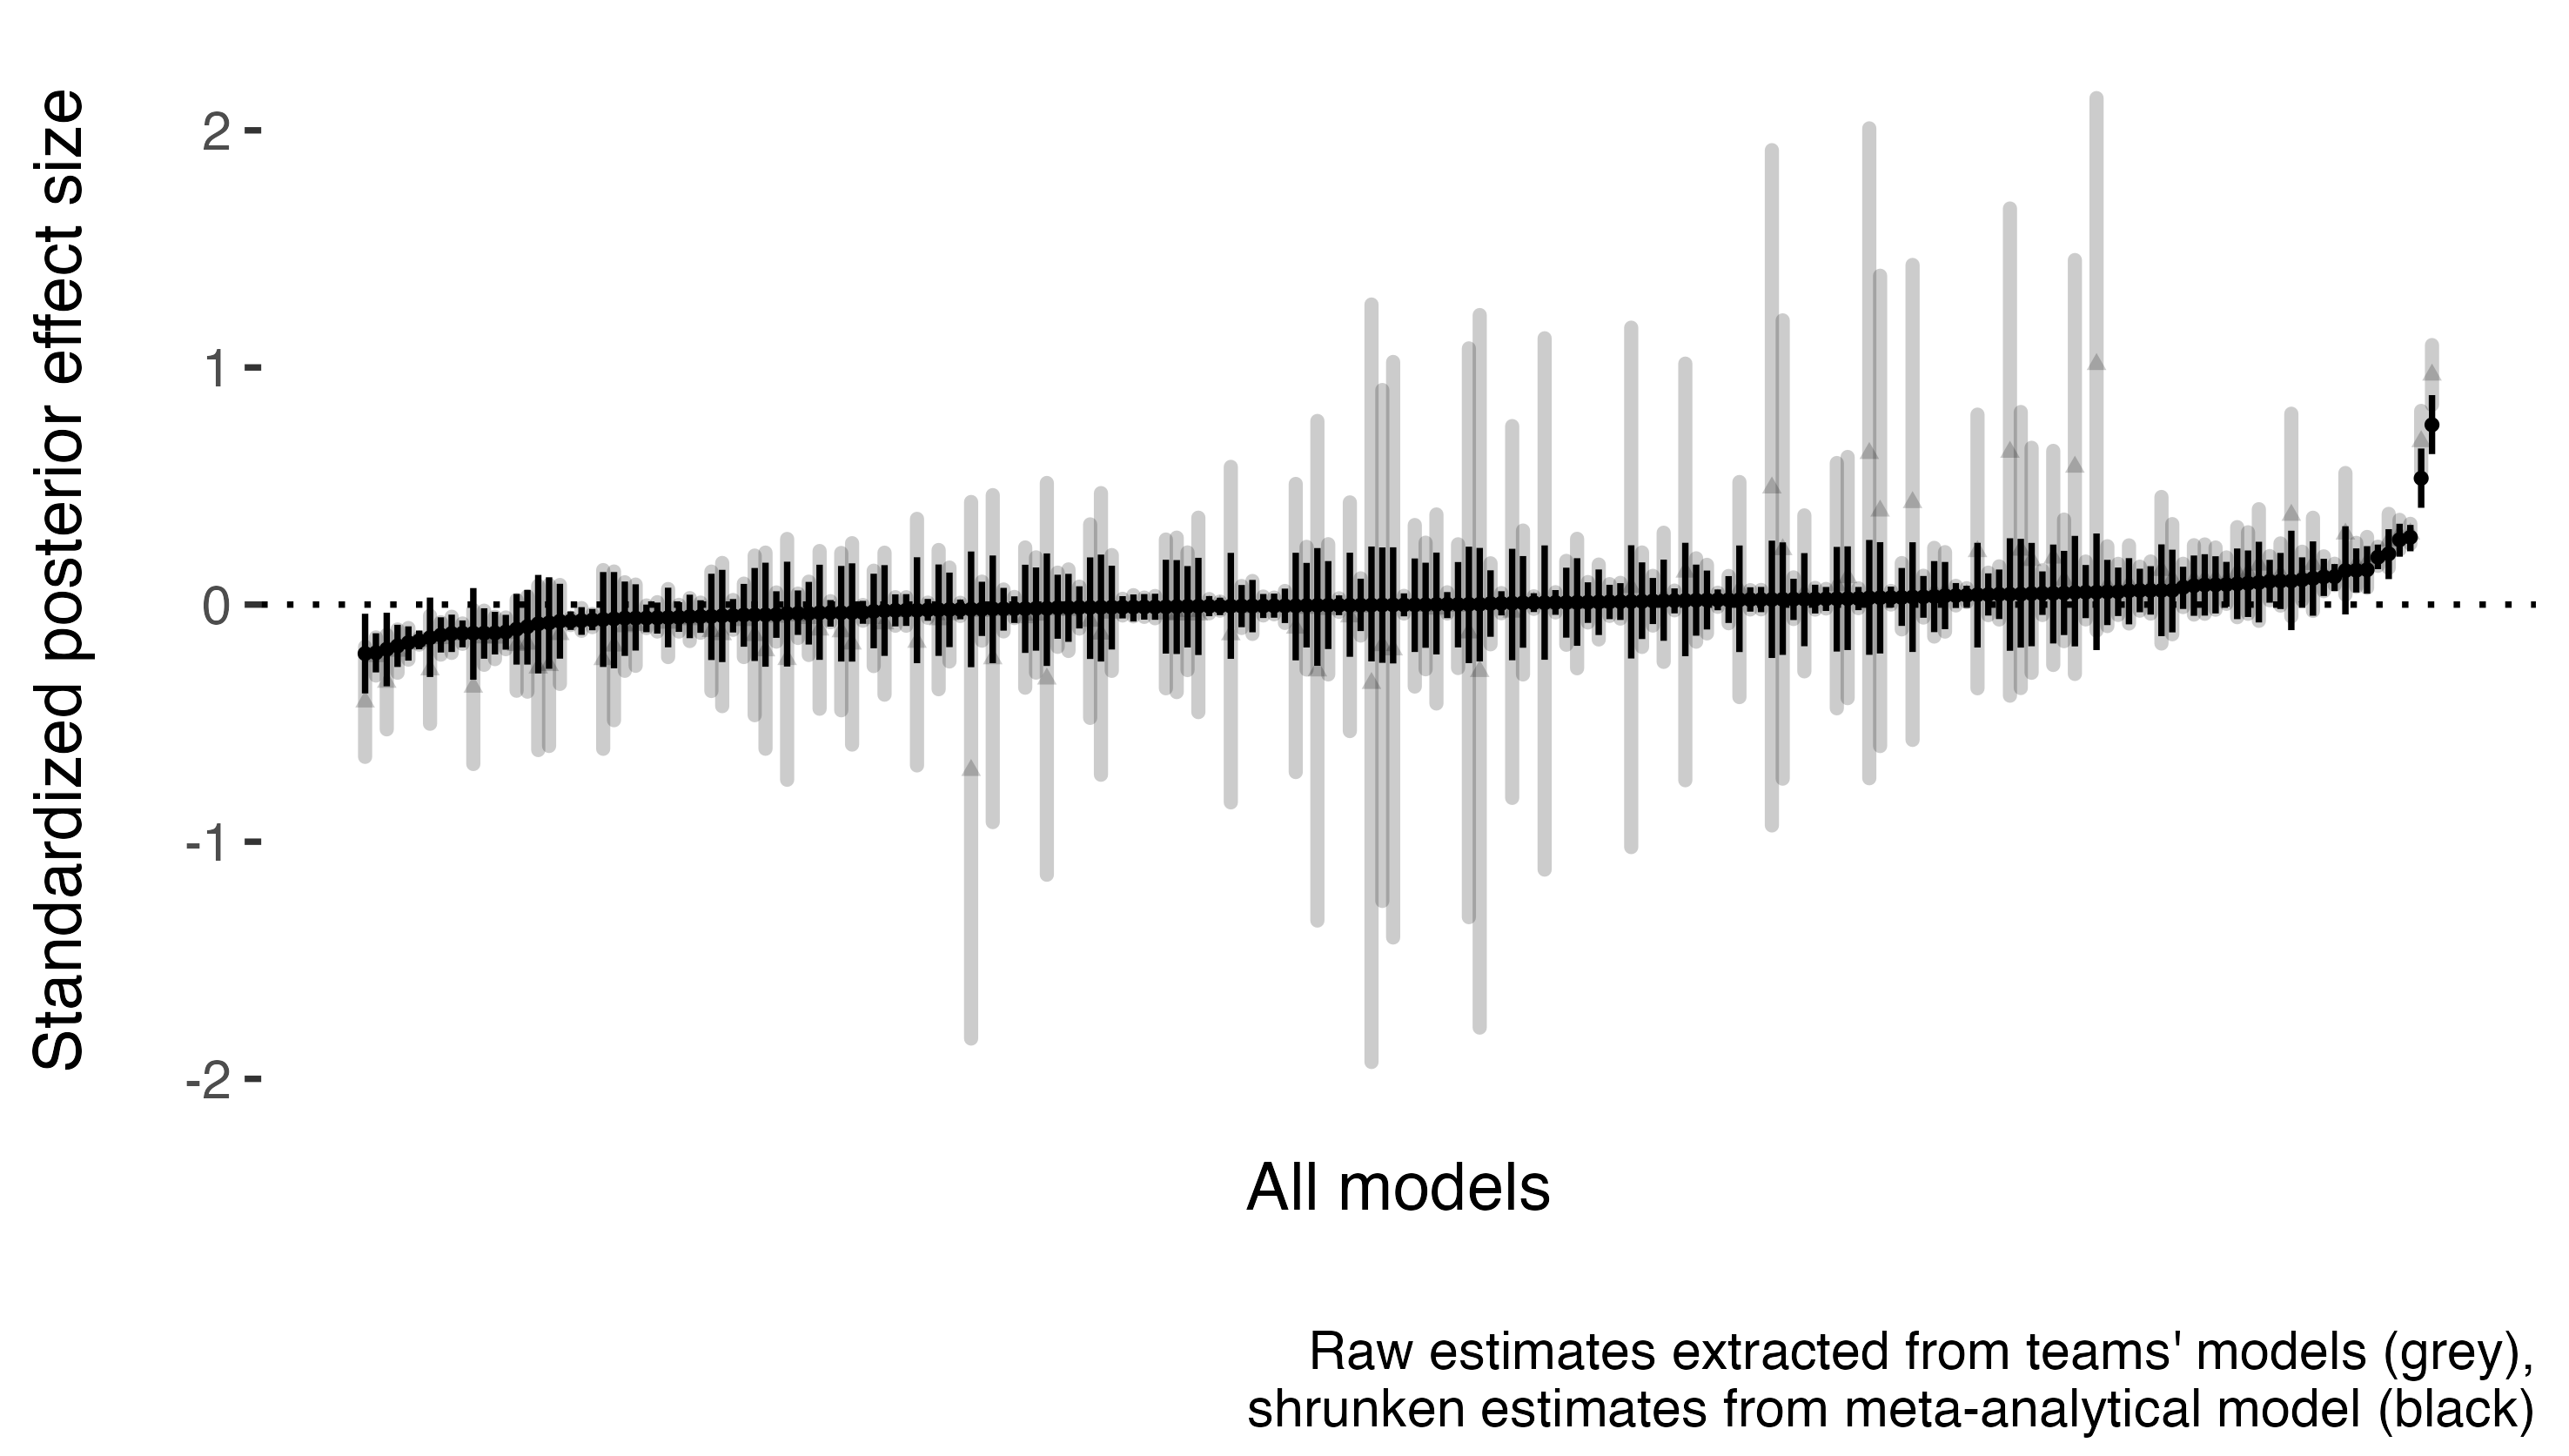
\includegraphics[width=1\linewidth]{../figs/meta_plot1_shrinkage} \caption{Standardized effect sizes across all critical coefficients provided by the teams. Raw estimates are displayed in grey. Estimates after shrinkage as provided by the meta-analytic model are displayed in black.}\label{fig:plot-meta1}
\end{figure}

\hypertarget{analytic-and-researcher-related-predictors}{%
\subsection{Analytic and researcher-related predictors}\label{analytic-and-researcher-related-predictors}}

After assessing the variability across teams and models, we now turn to estimating the impact of a series of predictors on the reported standardized effects.
There is a large amount of variation between and within teams, raising the question as to whether we can explain some of this variation or whether it is purely idiosyncratic \citep{breznau2021observing}.

We have run a model as described in Section Analytic and researcher-related predictors affecting effect sizes above.
Figure \ref{fig:plot-meta2}, panel C, displays the coefficients for all predictors alongside their 80\% and 95\% credible intervals.
The model suggests that most team-specific predictors yield very small deviations from the meta-analytic estimate and their 95\% credible intervals include zero, leaving us highly uncertain about their direction.
Neither analysts' prior beliefs in the phenomenon (\(\beta\) = -0.01, 95\% CrI = {[}-0.04, 0.01{]}), nor their seniority in terms of years after completing their PhD (\(\beta\) = 0.01, 95\% CrI = {[}-0.02, 0.04{]}) seem to affect model estimates.
Similarly, the evaluation of the quality of the analysis from their peers yielded a rather small effect magnitude, again characterized by large uncertainty (\(\beta\) = 0.02, 95\% CrI = {[}-0.01, 0.05{]}).
Interestingly, the model uniqueness, i.e.~how unique the choice and combination of predictors are, affects the analysts' estimate, with more unique models producing higher positive estimates (\(\beta\) = 0.04, 95\% CrI = {[}0.02, 0.07{]}).

Looking at the most important choices during measurement, both the acoustic parameter under investigation (e.g.~f0 or duration) and the choice of measurement window affected the results.
Panels A and B of Figure \ref{fig:plot-meta2} display the posterior estimates for the measurement outcome (i.e.~what acoustic dimension was measured, panel A) and measurement window (i.e.~what is the unit over which the outcome was measured, panel B).
If, on one hand, an acoustic dimension related to f0 was measured, estimates are lower than the meta-analytic estimate.
If, on the other hand, duration was measured, estimates are higher than the meta-analytic estimate.
Similarly, if acoustic parameters were measured across the entire sentence, estimates are lower than the meta-analytic estimate.
In other words, depending on the choice of measurement and the measurement window, analysts might have arrived at different conclusions about how and if typicality is expressed acoustically.

It is due of the latter patterns that we need to interpret the results of the model with great caution.
Since there are combinations of analytic choices that appear to systematically result in lower or higher estimates and the fact that predictors are not fully crossed (i.e.~we do not have the same amount of data for all combinations of e.g.~outcome and measurement window), the estimates for certain predictors might be biased if predictors are collinear.
This bias might be amplified by the fact that the scale has no natural way of being interpreted across all teams with different measurements cancelling each other out.
We checked correlations between predictors and while predictors do not seem to be highly collinear, the estimates might still be biased.



\begin{figure}
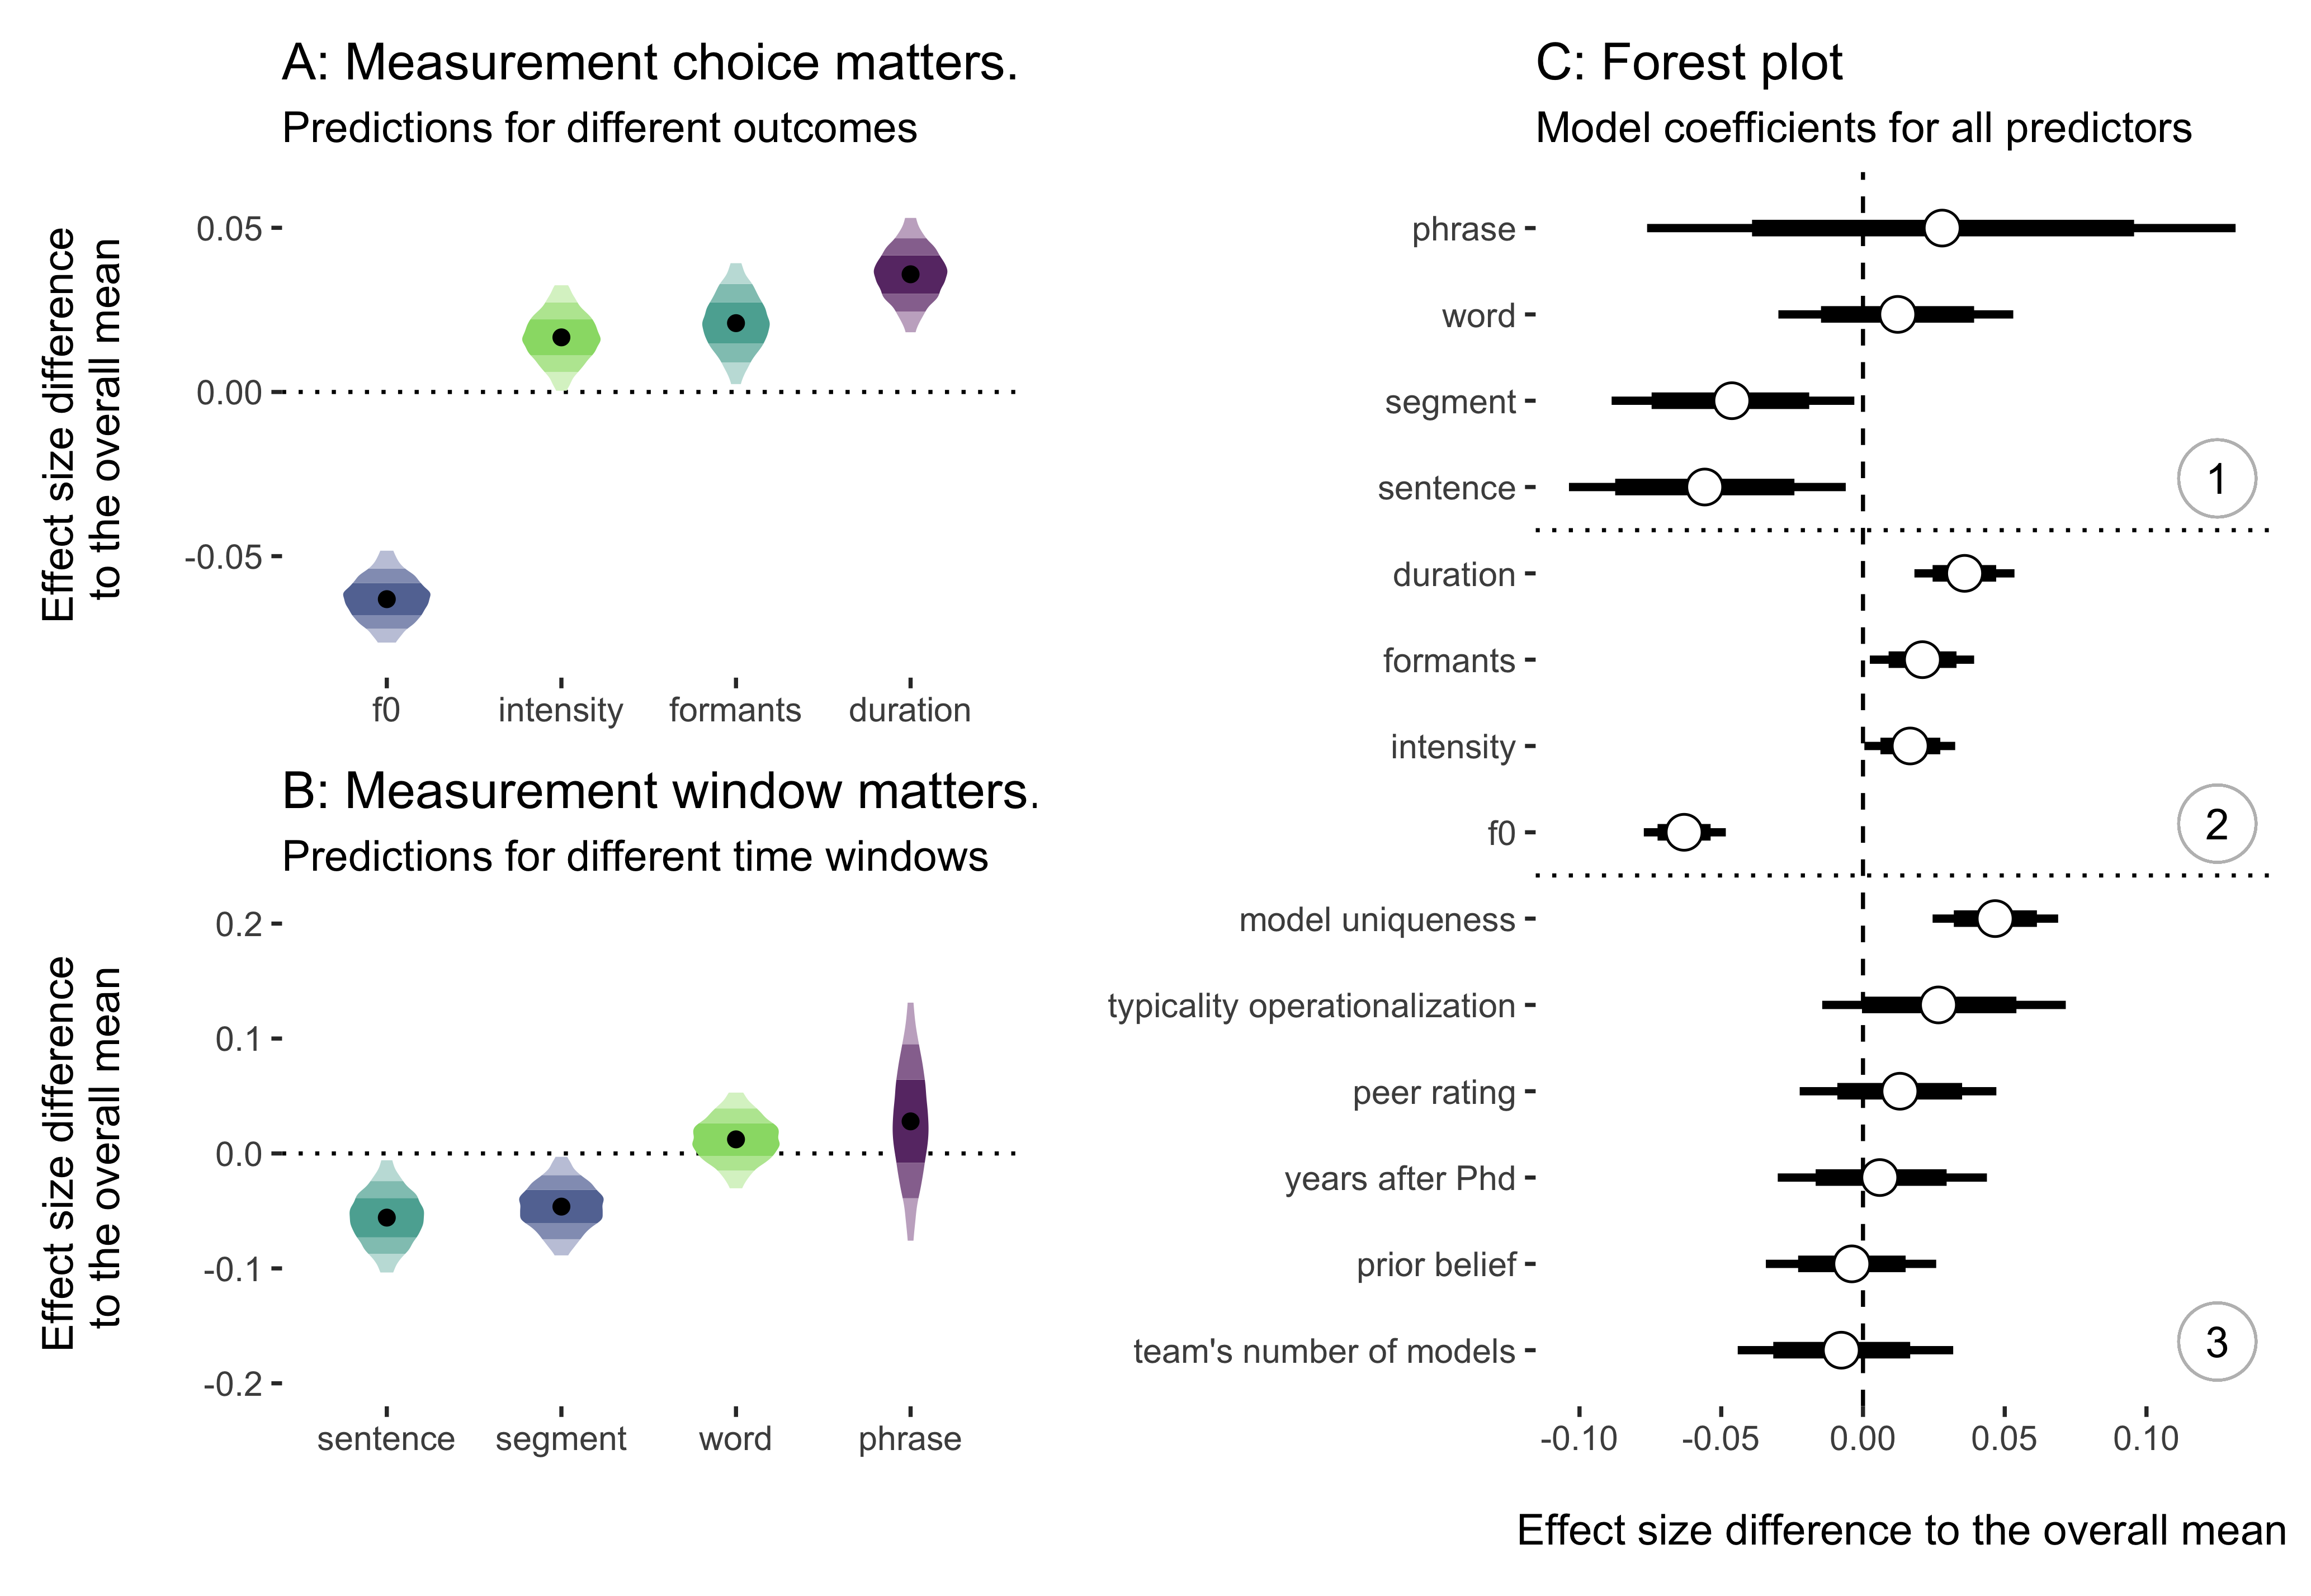
\includegraphics[width=1\linewidth]{../figs/alltogether} \caption{The effects of analytic and researcher-related predictors on the reported standardized effect sizes. (A) Posterior samples for the four most frequent outcome variables; (B) Posterior samples for the four most frequent temporal windows: Black points indicate medians; shaded areas represents 50/80/95\% highest density intervals. (C) Mean posterior samples (white circles) and 80/95\% credible intervals for all predictors grouped into predictors related to (1) temporal window, (2) outcome variable, and (3) team/analysis.}\label{fig:plot-meta2}
\end{figure}

\hypertarget{discussion}{%
\section{Discussion}\label{discussion}}

\hypertarget{summary}{%
\subsection{Summary}\label{summary}}

We gave 46 analyst teams the same speech data set to answer the same research question: \emph{Do
speakers acoustically modify utterances to signal atypical word combinations?}
In order to answer this question, teams had to interpret the research question by
operationalizing constructs within multidimensional signals, operationalizing and choosing appropriate model predictors, and constructing appropriate statistical models.
This complex process has led to a vast ``garden of forking paths'', i.e.~to a wide range of combinations of possible analytic decisions.
The submitted analyses exhibited at least 52 unique ways of operationalizing the acoustic signal alongside 55 unique ways of constructing the statistical model.
By multiplying the numbers of acoustic and model specifications, there are in principle 2860 possible unique combinations.
Note that this is a conservative estimate of the number of possible analytic choices for our research question, ignoring many other degrees of freedom like e.g.~acoustic parameter extraction, outlier treatment, and transformations, all of which might have an impact on the final results \citep{breznau2021observing}.

Different analysis paths led to different categorical conclusions with 39.4\% of teams reported to have found at least one statistically reliable effect.
To gain a better understanding of whether the observed quantitative variability can result in theoretically different claims, we will contextualize them in actual acoustic measures.
We calculated the standard deviation of a selection of acoustic measurements, as submitted by the analysis teams: duration, f0 and intensity, taken from different time windows.
These standard deviations can be considered as a coarse indication of the variability in the obtained acoustic measures.
We can now use these values to interpret the meta-analytic estimates, which are in standardized units, by transforming the standardized units to measures of duration, f0 and intensity.\footnote{Note that these categories necessarily refer to a variegated set of measures, for example the domain ``word'' includes words that differed along several dimensions, including their length and their metrical structure.}

For example, for those analyses that investigated the duration of vowels (e.g.~the duration of the stressed vowel in \emph{Banáne}), the reported duration measures exhibit standard deviations that range from 33.4 to 51.4 ms.
These standard deviations allow us to convert the meta-analytic estimates into milliseconds by multiplying those values with the the standard unit values of the meta-analytic estimates.
The reported effect estimates from teams varied between -0.7 and 1.01 standard units, which corresponds to estimated segment duration differences (for atypical vs typical combinations) ranging from -23.34 to 33.84 ms.
A more conservative approach is to convert the meta-analytic estimates of between-model variation, thus obtaining an estimate of between-model variability in milliseconds that ranges between 7.2 and 14.1 ms at 95\% credibility.
The calculation is thus: the minimum standard deviation of duration multiplied by the lower limit of the 95\% CrI of the between-models variability estimate, times 1.96 to obtain a 95\% CrI: 33.4 * 0.11 * 1.96 = 7.2 ms; the maximum standard deviation of duration multiplied by the upper limit of the 95\% CrI of the between-models variability estimate, times 1.96: 51.4 * 0.14 * 1.96 = 14.1 ms.

While this might not immediately strike one as highly variable, it crosses several theoretically relevant thresholds for perception and articulation:
for example, the widely studied phenomenon of incomplete neutralization involves vowel duration effects ranging from 7 to 15 ms \citep{nicenboim2018using}.
This particular phenomenon has sparked long-lasting methodological and theoretical debates about the very nature of linguistic representations \citep{port2005against} and has been replicated several times in both production and perception.
Vowel duration differences within this range have also been reported across phenomena associated with segmental contrasts \citep{coretta2019}, reduction phenomena \citep{nowak2006}, and biomechanical reflexes of prominence \citep{mucke2014effect}.
Thus, variation between different analyst teams of 7.2 to 14.1 ms in one or the other direction can be theoretically relevant and might lead to opposing theoretical conclusions.

\begin{table}

\caption{\label{tab:msa-sd-table}Estimated 95 percent CrIs of deviation from the meta-analytic effect in acoustic measures, based on the lower and upper limits of the between-model variation.}
\centering
\fontsize{11}{13}\selectfont
\begin{tabular}[t]{lllll}
\toprule
Outcome & Temporal window & Lower & Upper & Unit\\
\midrule
Duration & Segment & 7-10.8 & 9.3-14.4 & ms\\
Duration & Word & 6.9-25.3 & 9.1-33.4 & ms\\
f0 & Segment & 0.9-9.4 & 1.2-12.4 & hz\\
f0 & Word & 0.8-9.9 & 1.1-13.2 & hz\\
Intensity & Segment & 0.7-1.5 & 0.9-2 & dB\\
Intensity & Word & 0.7-0.9 & 1-1.2 & dB\\
\bottomrule
\end{tabular}
\end{table}

While one might find it obvious that measuring different parts of the speech signal can lead to different results, the fact that analysts (and reviewer alike) considered all these data analytic pipelines valid ways of answering the same research question points to a lack of theoretical consensus on what parts of the speech signal correspond to what types of communicative functions.
Importantly, even if analysts choose to measure more or less the same acoustic property within the same measurement window, they arrive at different estimates:
For example, five teams measured f0 in the noun and predicted f0 based on typicality as a categorical predictor. Their standardized effect estimates ranged from -0.35 to 0.19 standard deviations.
While these teams in principle measured the same thing, they differed in analytical details of how f0 was operationalized (i.e.~mean, minimum, maximum, point or range) and how their statistical model was constructed (i.e.~the number of predictors ranged from 1-2 and the number of random effect terms ranged from 1-10).
As shown by Breznau et al. \citeyearpar{breznau2021observing}, even seemingly inconsequential analytical choices can affect conclusions in non-trivial ways.

The observed variation does not seem to be systematic.
For example, variation between teams was not predicted by the analysts' prior expectations about the phenomenon.
In fact, teams on average rated the plausibility of the effect as rather high before receiving access to the data.
The observed variation was neither predicted by the analysts' experience in the field nor by the perceived quality of the analysis as judged by other teams.
Analyses received overall high peer-ratings for both the acoustic and the statistical analysis, suggesting that reviewers were generally satisfied with the other teams' approaches.

These findings are very much in line with previous crowd-sourced projects that suggest variation between teams is neither driven by perceived quality of the analysis nor by analysts' biases or experience \citep[e.g.,][]{silberzahn2018many, breznau2021observing}.
Following \citet[p.~9]{breznau2021observing}, we are bound to conclude that ``{[}\ldots{]} idiosyncratic uncertainty is a fundamental feature of the scientific process that is not easily explained by typically observed researcher characteristics or analytic decisions''.
Idiosyncratic variation across researchers might be a fact of life which we have to acknowledge and integrate into how we evaluate and present evidence.

While properties of the teams did not seem to systematically affect the results, teams' estimates seem to highly depend on certain measurement choices.
Human speech entails complex multidimensional signals.
Researchers need to make choices about what to measure, how to measure it and which temporal unit to measure it in.
Some of these choices seem to result in estimates in one direction while others seem to result in estimates into another.
For example, measurements related to f0 tended to result in lower estimates while measurements related to duration tended to yield higher estimates.

The asymmetry observed in the effect direction of different measurements can have several causes.
First, there could be a true underlying relationship between typicality and the speech signal that manifests itself in some measures but not others and/or manifests itself negatively in one acoustic measure but positively in another.

Secondly and orthogonal to a possible true relationship, certain measurement choices might be associated with stronger expectations relative to the research question, which might lead to stronger researcher biases.
Many analysts targeted measures related to f0, likely because similar functional relationships like information structure and predictability can be expressed by f0 \citep[e.g.][]{grice2017integrating, turnbull2017role}.
Moreover, prior work has actually suggested a relationship between typicality and f0 \citep[e.g.][]{dimitrova2008prosodic, dimitrova2009did}.
Participating analysts could have been aware of those findings, which might have, subconsciously or otherwise, nudged their choices into one particular direction.

Regardless of the cause of these systematic effects, we have to conclude that depending on the choice of how the speech signal is operationalized, researchers might find evidence for or against a theoretically relevant prediction.
This conclusion is further supported by the fact that between-team variability was lower than between-model variability.
This is an important observation when put into context of the fact that most teams submitted many different models.
Teams submitted up to 16 different models to test for a possible relationship between typicality and the speech signal.
The complexity of the speech signal lends itself to multiple approaches, but this plurality of hypothesis tests invites bias and can dramatically increase the rate of falsely claiming the presence of an effect \citep{roettger2019researcher, simmons2011false}.
We of course are not arguing that exploratory analyses should not be employed.
Rather, we simply want to point out that if the theoretical underpinnings of the field were much clearer, different teams would have converged towards a limited set of analyses despite of a less specific research question.

In relation to this aspect, one team coordinator decided to drop out of the project because of its approach being too top-down.
The coordinator also expressed a preference to be able to explore and run a variety of descriptive analyses followed up with inferential statistics.
We find that this attitude speaks to the main objective of the current study: investigate researchers' degrees of freedom in the speech sciences.
Based on our personal experience with research in the field, it is common practice to test many different types of models, using many different types of measurements, to answer one research hypothesis.
While this is a valid way to explore data and generate new hypotheses, it is not suitable for hypothesis testing.
When operating within the frequentist inferential framework, testing the same hypothesis with different dependent variables is known to increase the false-positive (Type-I error) rate.
The well-established solution to this problem is to apply a correction for family-wise error (i.e., alpha correction).
However, less clear-cut degrees of freedom such as observed in the present study can not be corrected for in a straightforward way.
If uncorrected for, these degrees of freedom can nevertheless drastically inflate the false positive rate, even if different choices are highly correlated \citep{roettger2019researcher}.
Another possible outcome of analytic flexibility as seen in this study is selective reporting of those tests that yield a desirable outcome \citep{kerr1998harking, john2012measuring, simmons2011false}, while null results remain unreported \citep{sterling1959publication, rosenthal1979file}.
Fields such as the speech sciences that make theoretical advances based on multidimensional data should be aware of this flexibility and calibrate their confidence in empirical claims accordingly.

Looking at our results, one might argue (and this interpretation has been articulated by several teams during the collaborative write-up) that our sample of speech scientists actually converged on a qualitative conclusion, i.e.~there is no evidence for a relationship.
However, if there truly was no underlying relationship, our results would suggest a concerning false positive rate with 39.4\% of teams reported to have found at least one statistically reliable effect.
This rate is substantially higher than the conventionally accepted 5\% false positive rate in for example null hypothesis significance testing frameworks.
If, on the other hand, there actually was an underlying relationship, our results would suggest a concerning false negative rate of -38.4\%, with the majority of teams not detecting the effect.
If the latter was true, the fact that the majority of teams arrived at a null result might also simply be a consequence of the sample size in the data set being too small to reliably detect an effect (which is unknown to us).
Thus, we do not think that our study provides convincing evidence that speech researchers converged on the same qualitative answer to a broad research question.

\hypertarget{lessons-for-the-methodological-reform-movement}{%
\subsection{Lessons for the methodological reform movement}\label{lessons-for-the-methodological-reform-movement}}

The current results point to important barriers to the successful accumulation of knowledge.
The replication crisis has brought attention to scientific practices that lead to unreliable and biased claims in the literature \citep{vazire2017quality, fidler2018reproducibility}.
One of the suggested paths forward is for researchers to directly replicate previous studies more often \citep{open2015estimating, camerer2018evaluating}.
While we agree with the importance of direct replications, our study (and similar crowd-sourced analyses before us) suggest that replicating more is simply not enough.
There is only limited value in learning that a particular procedure is replicable if the idiosyncratic nature of the procedure itself might not yield a representative result relative to all possible procedures that could have been applied to the research question.
Thus beyond a mere replication crisis, quantitative disciplines are going through an ``inference crisis'' \citep{rotello2015more, starns2019assessing}.
As shown by the peer-ratings of the analyses reported in this study, well-trained and experienced speech researchers not only applied completely different approaches to the same research question, but also considered most of these alternative approaches acceptable.
Being aware of this idiosyncratic variation between analysts should lead to more nuanced claims and a certain level of epistemic humility \citep[see][ for an overview of the concept]{campbell1975}.

A desired outcome of knowing that different but reasonable measurement choices or statistical approaches might lead to different interpretations of research data is to calibrate our (un)certainty in the strength of the collected evidence and, in turn, communicate that (un)certainty appropriately.
The fact that the choice of measurement, measurement window, and predictor choice affect the answer to the research question further suggests that research assumptions and hypotheses should be formulated in much greater detail, particularly so in regards to how measurement systems (here, the acoustic signal) and underlying conceptual constructs (here, the phonetic expression of typicality) relate to each other.

We should ideally specify the link between conceptual construct and quantitative system---the ``derivation chain'' \citep{dubin1970theory, meehl1990summaries}---prior to data collection and analysis, including defining constructs and their relationship within the quantitative system, specifying auxiliary assumptions and boundary conditions, and defining target measurements, statistical expectations and possible (and impossible) effect magnitudes.
Without well-defined derivation chains, we ``are not even wrong'' \citep{scheel2022most} because falsified expectations cannot tell us much about the conceptual constructs they are based on when the relationship between the two is underspecified.
Some of the analysis teams explicitly recognized and acknowledged the need to formulate a more precise version of the research question by preregistering their planned data analysis pipeline.
Preregistration, i.e.~a time-stamped document in which researchers specify how they plan to collect their data and/or how they plan to conduct their confirmatory analysis, is can be a useful tool to safeguard researchers against the urge to explore many different analytical paths before choosing the one that, in hindsight, seems most justified.
However, as long as the theoretical landscape does not allow for more precise hypotheses, the value of preregistration is limited and we need to find ways to appropriately calibrate the confidence in our claims.

Through sharing of materials, data and statistical protocols, we can make our idiosyncratic choices transparent to others \citep{munafo2017manifesto, vazire2017quality}.
Sharing further enables the evaluation and verification of underlying claims and allows for the evaluation of empirical, computational and statistical reproducibility \citep{lebel2018unified}.
It allows for alternative analyses to establish analytic robustness \citep{steegen2016increasing} and strengthens attempts to synthesize evidence via meta-analyses \citep[e.g.,][]{nicenboim2018using}.
Given that minor procedural changes can sometimes drastically affect the final interpretation of the results \citep{breznau2021observing}, we should ideally share a detailed documentation of the data collection procedure, the measurement choices, the data extraction, and statistical analyses.
Within fields that deal with speech data, open source software that permits the extraction of acoustic parameters via reproducible scripts can help other researchers to trace back seemingly inconsequential choices during the measurement process \citetext{\citealp[e.g., Praat:][]{boersma2021praat}; \citealp[EMU:][]{winkelmann2017emu}; \citealp[the Montreal Forced Aligner:][]{mcauliffe2017}}.

Making analytic pathways completely re-traceable and preregistering them in advance does not change the fact that different analysts might apply different analytic approaches (preregistered or not).
Crowd-sourced projects such as the current one can shed light on the range of degrees of freedom during analysis and could possibly help produce a consensual estimated effect if the research hypothesis is specific enough.
Crowd-sourcing analyses is obviously not always feasible in terms of required resources and time, but could be a consideration for claims that have large epistemological or practical consequences.

If we develop a good understanding of relevant analytic degrees of freedom, we could apply all conceivable analytic strategies and compare the results across all combinations of these choices.
Such an analysis can provide insight into how much the conclusions change due to analytic choices as well as which choices have neglible or large impact on the result.
This approach is called a ``multiverse analysis'' \citep[e.g,][]{steegen2016increasing, harder2020multiverse} and has recently gained popularity across disciplines.

Finally, neither crowd-sourcing nor multiverse analyses will guarantee that all relevant pathways are explored.
Crowd-sourcing is limited by the sampled analysts and their biases.
Multiverse analyses are limited even further by the group of researchers who define possible analytic pathways.
Eventually, a mature scientific discipline needs to develop a set of detailed quantitative hypotheses of how conceptual constructs manifest themselves in the measured system, i.e.~in the present case how communicative pressures of certain functions are expressed in the acoustic signal.
Possible tools to strengthen theoretical development relate to mathematically formalizing verbal expectations or using computational models \citep[e.g.,][]{van2020formalizing, guest2021computational, scheel2021hypothesis, devezer2021case}.
Although conceptually promising, in their current state, such formalized models typically work in spaces that are much lower in dimensionality than the complex systems in which we measure. Thus, future research should spend resources on attempting to quantitatively relate the abstract theoretical space to the complex measurement space.

\hypertarget{caveats}{%
\subsection{Caveats}\label{caveats}}

Our study has several limitations that need to be considered when interpreting our results.

First, while the total number of analyses is larger than most earlier crowd-sourcing projects, it is likely to be too small to reliably estimate the impact of certain predictors.
Since predictors' values were not systematically distributed across teams, our estimates are characterized by large uncertainty.

Second, uncertainty is further inflated by the fact that the research question presented to the teams was vague, despite being of a kind normally found in the speech science literature: \emph{Do speakers acoustically modify utterances to signal atypical word combinations?}
Interpreting the research question/hypothesis differently in terms of its statistical consequences has recently been shown to explain some variation between analysis teams in many-analyses projects \citep{auspurg2021has}.
The analysts might also have tried to answer different specific manifestations of the research question that was given to them, leading to different choices down the line (e.g.~Do speakers modify f0 in atypical adjectives?).
It could be argued that some teams would have not specified such a vague research question to begin with which would have reduced the possible degrees of freedom substantially.
However, this very underspecification of research hypotheses in the field of speech science \citep[and beyond, see][]{scheel2022most} is very common.
For example, researchers seem to have not yet agreed on how to acoustically measure cross-linguistically common phenomena such as word stress \citep[e.g.][]{gordon2017acoustic}.
Research on acoustic markers of clinical conditions such as depression and schizophrenia are often difficult to compare due to the wide variety of different acoustic measures employed \citep[e.g.][]{cummins2015review, parola2022speech}.

Third, the design of this crowd-sourced study has artificially inflated the variability between teams by encouraging anti-coordination strategies.
Teams knew that there will other analyst teams and therefore might have chosen a ``less canonical'' analysis.
Since analysts were guaranteed to become co-authors of a (in principle) guaranteed publication, such an anti-coordination approach was not explicitly disincentivized.

Forth, our sample is an opportunity sample.
We have advertised the project through online platforms which might have led to the exclusion of certain potential researcher groups.
The sampling strategy also might have given access to researchers who were less experienced in particular aspects of the data analysis, possibly introducing uncommon analytic choices or poor quality analyses.
However, to our knowledge, neither the peer review among teams nor the information gathered through our questionnaires indicated any obvious cases of what one might consider incompetent analyses.

In light of both the observed large variability between teams, and possible sources of bias, a field can benefit from explicit positionality statements \citep[e.g.,][]{jafar2018, darwin2020, fox2021open}.
Researchers do not analyze data in a vacuum.
It is important to recognize and disclose one's positionality, i.e., a reflection about how educational background, social identity, power, experience and context might influence researchers' approaches and interpretations.
For example, the coordinating authors have engaged with meta-scientific research before and have been actively involved in methodological debates about scientific practices including transparency and statistical methods.
They have in the past used the lack of standardized analytic approaches as an argument for proposing behavior and policy changes in the field.
This might have biased their own judgement during the analysis which itself came with many researcher degrees of freedom.
We hope we were able to make these degrees of freedom as well as the timing and reasoning of these analytic choices at least detectable and we invite other researchers to re-analyze our data and try to replicate our results using a different research question.

Finally, the present study focused on a particular phenomenon within the speech sciences using a speech production data set with very specific properties.
The generalizability of our findings to other disciplines, as well as to other sub-disciplines of the language sciences specifically, is, of course, limited.
We focused on quantitative analyses that require the operationalization of a multidimensional signal in an artificial elicitation situation (laboratory speech).
While we do believe that our qualitative conclusions hold across fields exhibiting similar methodologies, the detailed quantitative results will only be able to directly inform similar disciplines that work with speech or audio/video signals.
This is an important point to make because cognitive sciences in general, and the language sciences in particular, have many research areas that are based on qualitative methods \citep{haven2019}.
It is conceivable that the discussed issues apply differently or not at all to qualitative data analyses.

\hypertarget{conclusion}{%
\section{Conclusion}\label{conclusion}}

In recent efforts, several studies have highlighted the large degree of analytic flexibility in data analysis.
When many different analysts have to analyze the same data set to answer the same research question, analysts differ in how they approach this task, leading to both different qualitative answers (i.e.~is there evidence for a relationship or not) and different effect magnitudes.
This is concerning, as it can lead to substantially different conclusions based on the same data set, a state of affairs that can generate biased inferential decisions and might weaken confidence in the published literature.
More specifically, what we find of particular relevance is the fact that commonly research proceeds based on publications from one research team at a time.
If we imagine a situation where any of the 46 teams could have been \emph{the} team publishing a study on this topic, it is immediately clear that that single study is just a very limited view.
In light of this we want to stress that the field has to quickly move from one-off studies to collaborative approaches like the one employed here and to more frequent replication attempts for example by incentivizing replication through dedicated funding and editorial policies, among others.

Going beyond previous empirical studies, the current paper looked at many analyses of speech data.
Speech is a multidimensional signal that allows for great flexibility because it lends itself to a variety of possible operationalizations.
In this study, 46 teams of speech scientists analyzed the same data set.
Analytic approaches differed vastly in terms of their operationalization of key constructs, as well as their statistical analyses.
Given the observed variability, conservative estimates of the sheer number of possible analytic paths for this research question lies in the thousands.
Quantitatively, the between-team and between-model variation of estimates crosses important theoretical thresholds as to what constitutes communicative, cognitive, or bio-mechanical values.

In line with previous findings, neither the perceived quality of analyses, nor the experience or prior beliefs of teams explained the observed variation.
Importantly however, we found some evidence for systematic effects on teams' estimates based on what and how they measured the speech signal.
This result, taken together with the meaningful between-model variation and the tendency to test the research question on multiple outcome variables, suggests that a vast plurality of acceptable approaches is expected to frequently lead to different conclusions.
We suggest that fields that use multidimensional data need to acknowledge these degrees of freedom, consider crowd-sourcing and multiverse analyses when evaluating epistemologically or practically important phenomena, and strengthen the link between theoretical predictions and the measurement system by means of mathematical formalization and computational modeling.

\hypertarget{author-contributions}{%
\section{Author contributions}\label{author-contributions}}

See \url{https://github.com/many-speech-analyses/many_analyses/blob/main/figs/credit-taxonomy-all.png}.

\hypertarget{conflicts-of-interest}{%
\section{Conflicts of interest}\label{conflicts-of-interest}}

We have no conflicts of interest to disclose.

\hypertarget{acknowledgements}{%
\section{Acknowledgements}\label{acknowledgements}}

We would like to thank the editors David Sbarra and Julia Strand, Matthew Goldrick and two anonymous reviewers for their insightful comments and suggestions.

The initiating authors (SC, JVC, TR) wish to express immense gratitude to all the other authors, without which this project would not have come to be.

All remaining errors are the initiating authors' (SC, JVC, TR)

\hypertarget{funding}{%
\section{Funding}\label{funding}}

Stefano Coretta was partially supported by the European Research Council Grant No.~742289 Human interaction and the evolution of spoken accent (2017--2022) awarded to Prof.~Jonathan Harrington.

Jalal Al-Tamimi was partially supported by the French Investissements d'Avenir - Labex EFL program (ANR-10- LABX-0083), contributing to the IdEx Université Paris Cité - ANR-18-IDEX-0001.

George Moroz, Sita Carraturo: The research leading to these results has received funding from the Basic Research Program at the National Research University Higher School of Economics.

Iñigo Urrestarazu-Porta: The research leading to these results has received funding from the MADPAB (National Research Agency of the French republic, ANR-20-CE27-0007) and Monumenta Linguae Vasconum 6: avances en la cronología de la historia y la prehistoria de la lengua vasca projects (Ministry of Science and Innovation of the Spanish kingdom, PID2020-118445GB-I00).

Constantijn Kaland, Martine Grice: German Research Foundation (DFG) - Project-ID 281511265 - SFB 125.

Nina R. Benway: This research was supported in part through computational resources provided by Syracuse University (NSF ACI-1341006; NSF ACI-1541396).

\appendix

\hypertarget{glossary}{%
\section{Glossary}\label{glossary}}

\begin{itemize}
\tightlist
\item
  \textbf{Analysis team}: team of analysts or single analyst.
\item
  \textbf{Reported effect sizes}: effect sizes reported by each analysis team.
\item
  \textbf{Standardized model}: Bayesian refit of the team's model.
\item
  \textbf{Standardized effect sizes}: (\(\eta_i\)) effect sizes returned by the standardized models.
\item
  \textbf{Standardized standard error}: (\(\text{se}_i\)) standard deviation of the standardized effect sizes.
\item
  \textbf{Bayesian random-effects meta-analysis} and \textbf{meta-analytic model}: multilevel intercept-only regression model for meta-analysis.
\item
  \textbf{Meta-analytic group-level standard deviation}: (\(\sigma_{\alpha_{\text{t}}}\)) standard deviation of the group-level effect of team returned by the meta-analytic model.
\item
  \textbf{Analytic and researcher-related predictors}: predictors used in the model that assess the effect of analytic and researcher-related factors on the standardized effects.
\end{itemize}

\bibliographystyle{sageh}
\bibliography{references}


\end{document}
